
\section{Multi-task Sequence to Sequence Learning}
Multi-task learning (MTL) is an important machine learning paradigm that
aims at improving the generalization performance of a task using other related
tasks. 
Such framework has been widely studied by
\newcite{thrun96,caruana97,evgeniou04,ando05,argyriou07,kumar12}, among many
others. In the context of deep neural networks, MTL has
been applied successfully to various problems ranging from language
\cite{liu15}, to vision
\cite{donahue14},
and speech \cite{heigold13,huang2013cross}.

\begin{sloppypar}
Recently, sequence to sequence (\ssl{}) learning
\cite{kal13,sutskever14,cho14} emerges as an effective paradigm for dealing with
variable-length inputs and outputs. \ssl{} learning, at its core, uses
recurrent neural networks to map variable-length input sequences to
variable-length output sequences.  While relatively new, the \ssl{}
approach has achieved state-of-the-art results in not only its original
application -- machine translation --
\cite{luong15,jean15,luong15attn,jean15wmt,luong15iwslt}, but also image caption generation \cite{vinyals15caption},
and constituency parsing \cite{vinyals15grammar}. 
\end{sloppypar}

Despite the popularity of multi-task learning and sequence to sequence
learning, there has been little work in combining MTL with \ssl{}
learning. To the best of my knowledge, there is only one recent
publication by \newcite{dong15} which applies a \ssl{} models for machine
translation, where the goal is to translate from one language to
multiple languages.
In this work, I propose three MTL
approaches that complement one another: (a) the {\it \otm} approach -- for
tasks that can have an encoder in common, such as translation and parsing; this 
applies to the multi-target translation setting in \cite{dong15} as well, (b)
the {\it \mto} approach -- useful for multi-source
translation or tasks in which only the decoder can be easily shared,
such as translation and image captioning, and lastly, (c) the {\it \mtm} approach -- which share
multiple encoders and decoders through which I study the effect of unsupervised
learning in translation.
I show
that syntactic parsing and image caption generation improves the
translation quality between English and German by up to +$1.5$ BLEU points over
strong single-task baselines on the WMT benchmarks. 
Furthermore, I have established a new {\it state-of-the-art} result in
constituent parsing with 93.0 F$_1$.
I also explore two unsupervised learning
objectives, sequence autoencoders \cite{dai15} and skip-thought vectors
\cite{kiros15skip}, and reveal their interesting properties in the MTL setting: autoencoder helps less in terms of
  perplexities but more on BLEU scores compared to skip-thought.
%My novel findings reveal that the skip-thought objective improves
%translation while the sequence autoencoders does not.
\begin{figure}%[tbh]
\centering
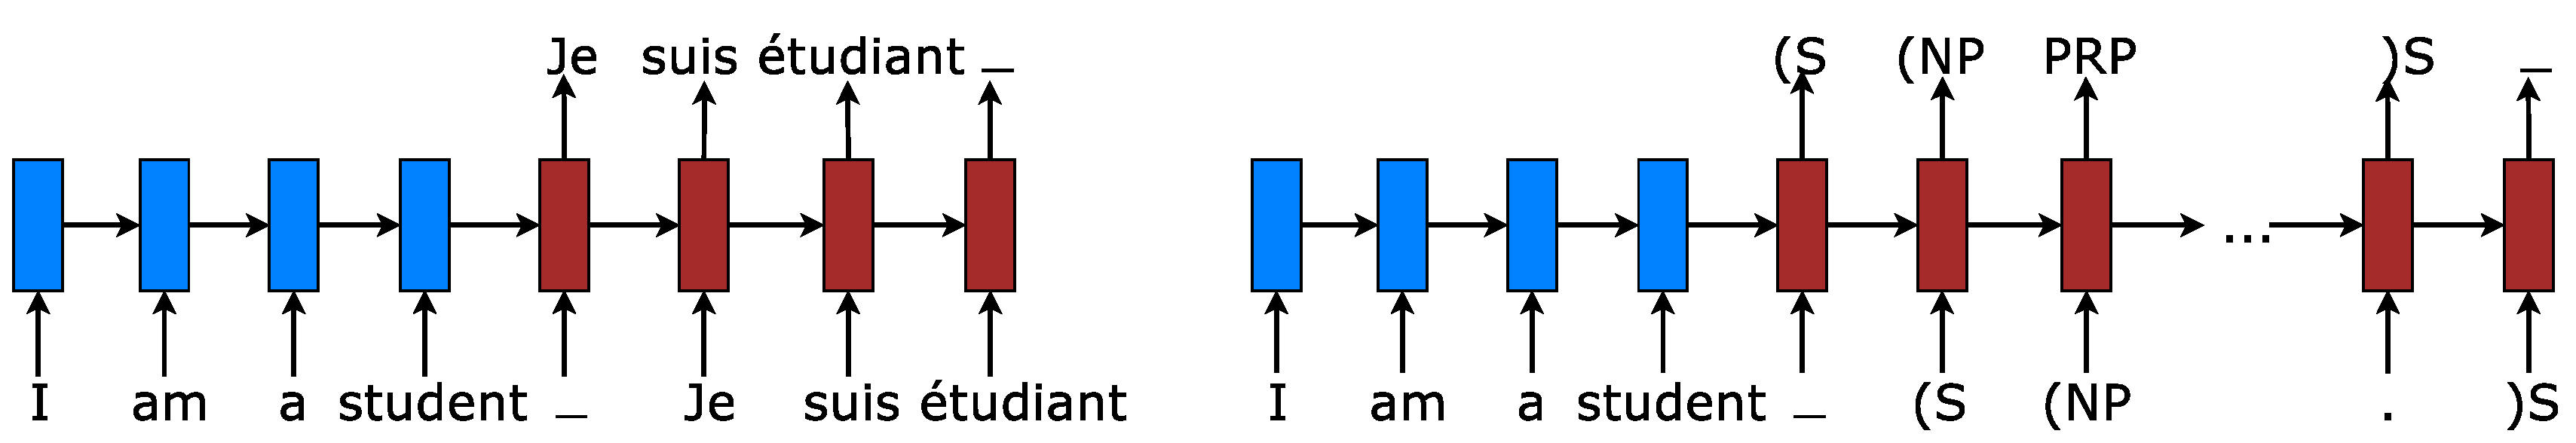
\includegraphics[width=1\textwidth, clip=true, trim= 0 0 0
0]{img/6-1_seq2seq}
\caption[Sequence to sequence learning examples]{{\bf Sequence to sequence learning examples} -- (left) machine
translation \cite{sutskever14} and ({\it right}) constituent parsing
\cite{vinyals15grammar}.}
\label{f:s2s}
\end{figure}



\begin{figure}%[tbh]
\centering
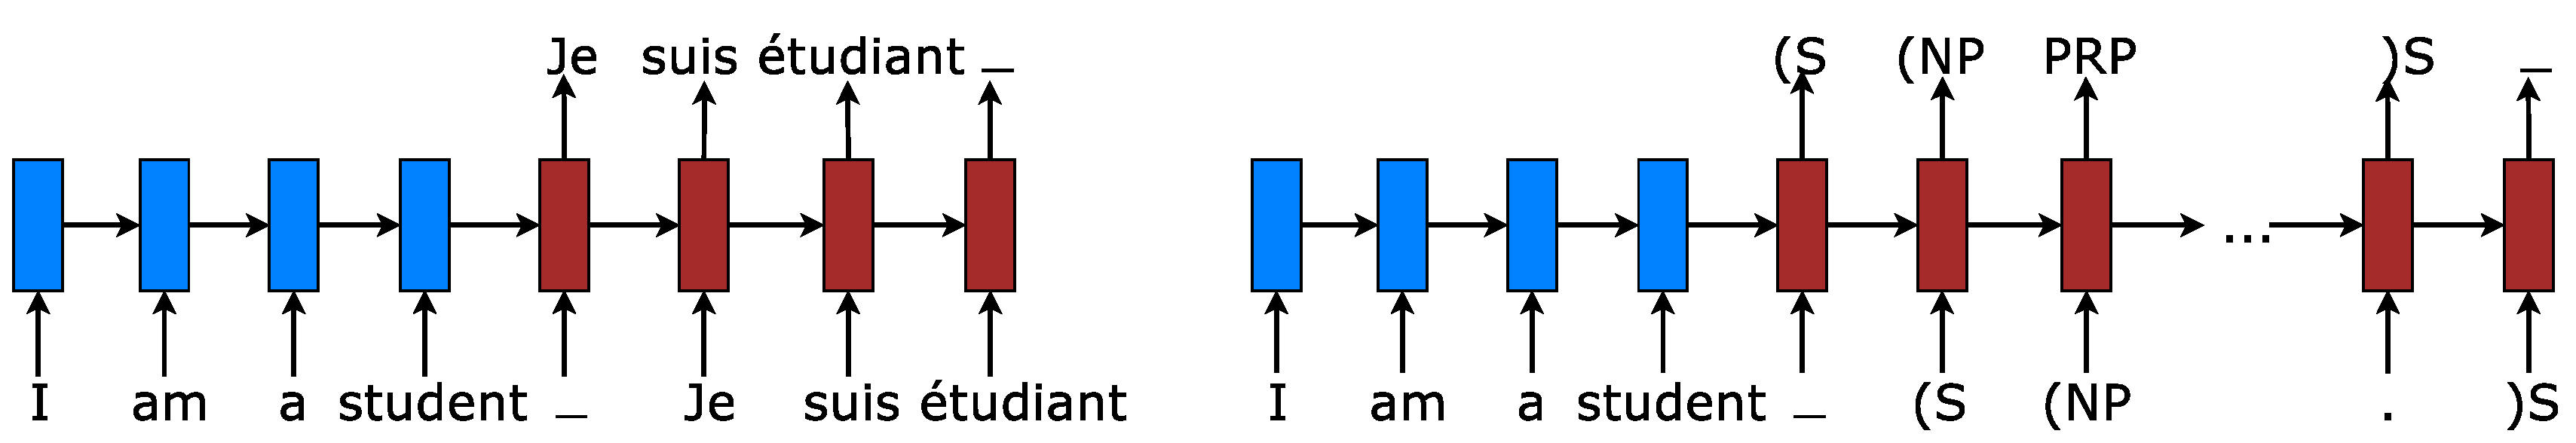
\includegraphics[width=1\textwidth, clip=true, trim= 0 0 0
0]{img/6-1_seq2seq}
\caption{{\bf Sequence to sequence learning examples} -- (left) machine
translation \citep{sutskever14} and ({\it right}) constituent parsing
\citep{vinyals15grammar}.}
\label{f:s2s}
\end{figure}


\subsection{Multi-task Sequence-to-Sequence Learning}
\label{subsec:multi}
We generalize the work of \citet{dong15} to the multi-task sequence-to-sequence
learning setting that includes the tasks of machine translation (MT),
constituency parsing, and image caption generation. Depending which tasks 
involved, we propose to categorize multi-task \ssl{} learning into three general
settings.
In addition, we will discuss the unsupervised learning tasks considered as well
as the learning process.

\paragraph{One-to-Many Setting}
%\label{subsec:otm}
This scheme involves {\it one encoder} and {\it multiple decoders} for tasks in
which the encoder can be shared, as illustrated in
Figure~\ref{f:otm}. The input to each task is a sequence of
English words. A separate decoder is used to generate each sequence of
output units which can be either (a) a sequence of tags for
constituency parsing as used in \citep{vinyals15grammar}, (b) a
sequence of German words for machine translation \citep{luong15attn},
and (c) the same sequence of English words for autoencoders or a
related sequence of English words for the skip-thought objective
\citep{kiros15skip}.

\begin{figure}[tbh]
\centering
%\psgrid
%\rput(7.5,2.6){$\alpha_1=1.0$}
%\rput(7.5,1.5){$\alpha_2=0.1$}
%\rput(7.5,0.4){$\alpha_3=0.5$}
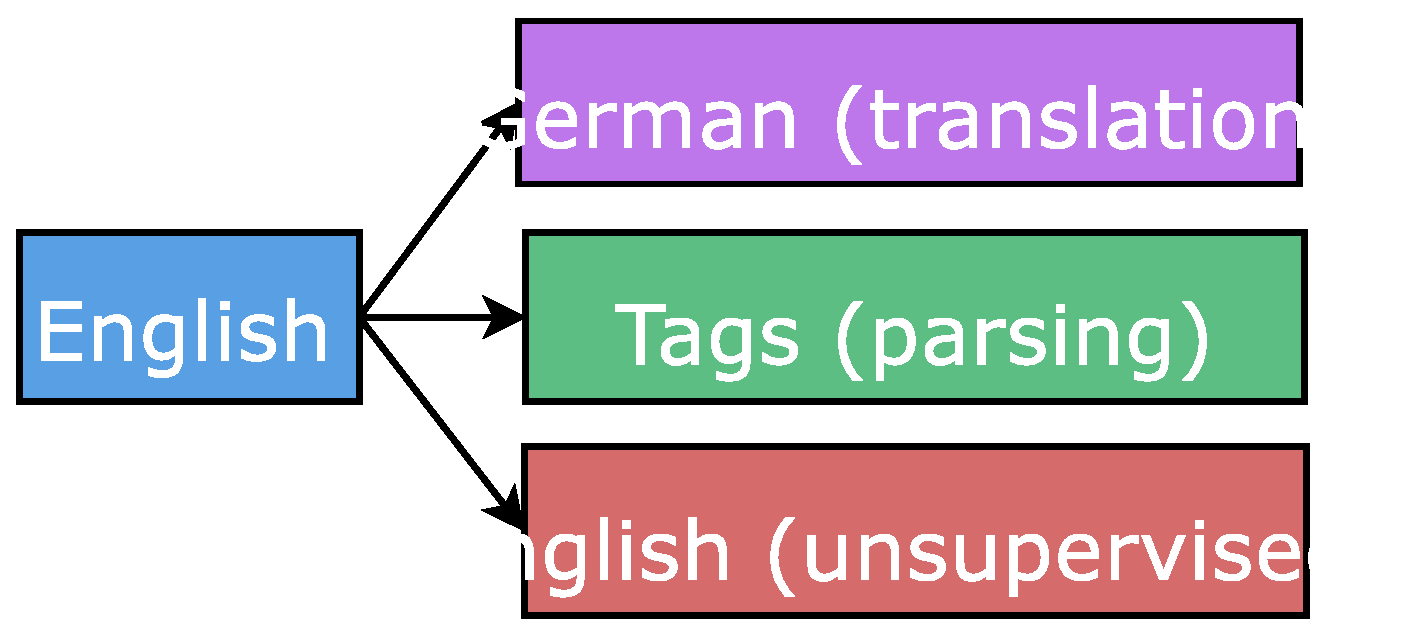
\includegraphics[width=0.45\textwidth, clip=true, trim= 0 0 0
0]{img/6-1_otm}
\caption[One-to-many Setting]{{\bf One-to-many Setting} -- one encoder, multiple decoders. This scheme
is useful for either multi-target translation as
in \cite{dong15} or between different tasks. Here, English and
German imply sequences of words in the respective languages. 
%The $\alpha$ values
%give the proportions of parameter updates that are allocated for the different tasks.
} 
\label{f:otm}
\end{figure}

\paragraph{Many-to-One Setting}
%\label{subsec:mto}
This scheme is the opposite of the {\it one-to-many}
setting. As illustrated in Figure~\ref{f:mto}, it consists of {\it multiple
encoders} and {\it one decoder}. This is useful for tasks in which only the
decoder can be shared, for example, when our tasks include machine translation
and image caption generation \citep{vinyals15caption}. In addition, from a machine
translation perspective, this setting can benefit from a large
amount of monolingual data on the target side, which is a standard
practice in machine translation system and has also been explored
for neural MT by \cite{gulcehre2015using}.

\begin{figure}[tbh]
\centering
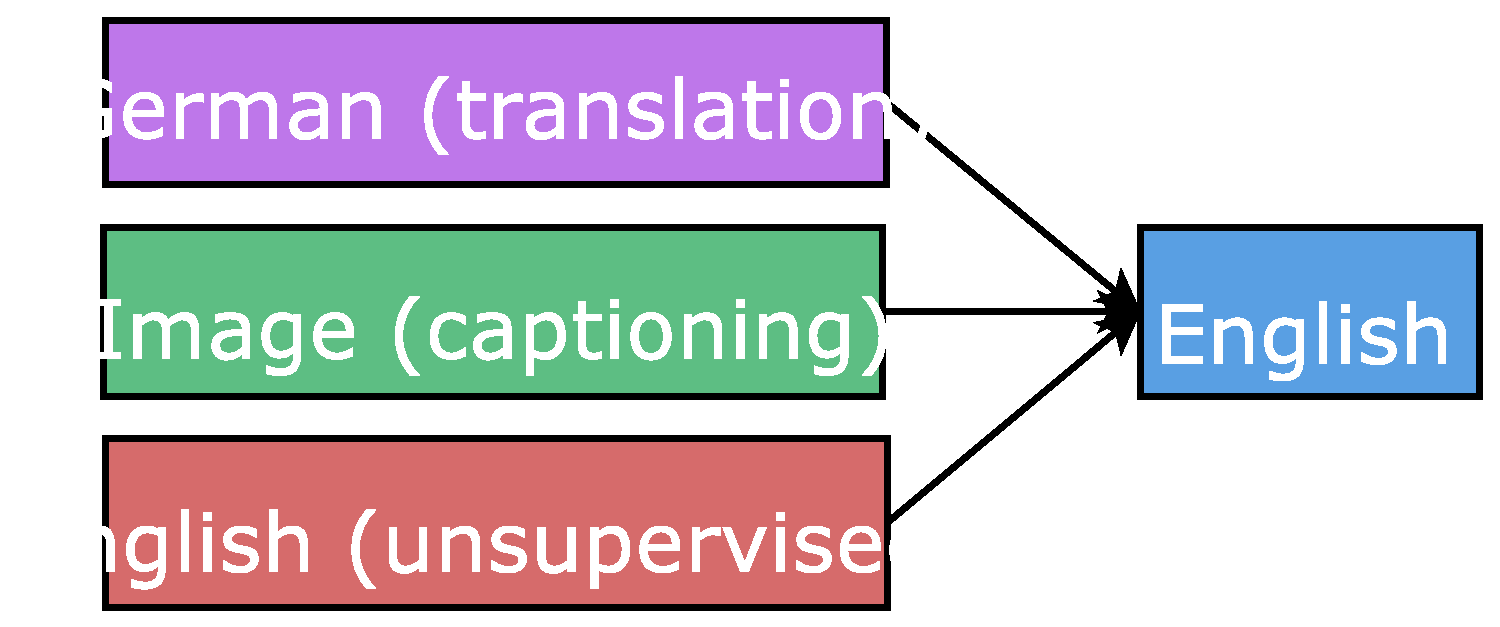
\includegraphics[width=0.5\textwidth, clip=true, trim= 0 0 0
0]{img/6-1_mto}
\caption[Many-to-one setting]{{\bf Many-to-one setting} -- multiple encoders, one decoder. This scheme
is handy for tasks in which only the decoders can be shared.}
\label{f:mto}
\end{figure}

\paragraph{Many-to-Many Setting}
%\label{subsec:mtm}
Lastly, as the name describes, this category is the most general one,
consisting of multiple encoders and multiple decoders.
%However, such
%flexibility also makes it difficult to determine which tasks should
%share which components. ---- Is it true? IS. 
%To simplify sharing, we consider a special use
%case in machine translation which involves two encoders and two
%decoders shared over three tasks.
We will explore this scheme in a translation setting that involves sharing multiple
encoders and multiple decoders.  In addition to the machine
translation task, we will include two unsupervised 
objectives over the source and target languages as illustrated in
Figure~\ref{f:mtm}.

\begin{figure}[tbh]
\centering
\includegraphics[width=0.7\textwidth, clip=true, trim= 0 0 0
0]{img/6-1_mtm}
\caption[Many-to-many setting]{{\bf Many-to-many setting} -- multiple encoders, multiple decoders. We
consider this scheme in a limited context of machine translation to utilize the large
monolingual corpora in both the source and the target languages. Here, we
consider a single translation task and two unsupervised autoencoder tasks.} 
\label{f:mtm}
\end{figure}

\paragraph{Unsupervised Learning Tasks}

Our very first unsupervised learning task involves learning {\it autoencoders} from
monolingual corpora, which has recently been applied to sequence to sequence
learning \citep{dai15}. However, in \citet{dai15}'s work, the authors
only experiment with pretraining and then finetuning, but not joint training which
can be viewed as a form of multi-task learning (MTL). As such, we are
very interested in knowing whether the same trend extends to our MTL settings.

Additionally, we investigate the use of the {\it skip-thought}
vectors \citep{kiros15skip} in the context of our MTL framework.
Skip-thought vectors are trained by training sequence to sequence
models on pairs of consecutive sentences, which makes the skip-thought
objective a natural \ssl{} learning candidate. A minor technical
difficulty with skip-thought objective is that 
the training data must consist of ordered sentences, e.g., paragraphs.  Unfortunately, in
many applications that include machine translation, we only have
sentence-level data where the sentences are unordered. To
address that, we split each sentence into two halves; we then use 
one half to predict the other half.

\paragraph{Learning}
%\label{subsec:learning}
\cite{dong15} adopted an {\it alternating} training approach, where they
optimize each task for a fixed number of parameter updates (or
mini-batches) before switching to the next task (which is a different
language pair). In our setting, our tasks are more diverse and contain
different amounts of training data. As a result, we allocate different
numbers of parameter updates for each task, which are expressed with
the {\it mixing} ratio values $\alpha_i$ (for each task $i$). Each
parameter update consists of training data from one task only. When
switching between tasks, we select randomly a new task $i$ with
probability $\frac{\alpha_i}{\sum_j \alpha_j}$.
%{\bf [Thang, make sure that it is correct]} 


Our convention is that the first task is the
{\it reference} task with $\alpha_1 = 1.0$ and the number of training
parameter updates for that task is prespecified to be $N$. A typical task $i$ will then be
trained for $\frac{\alpha_i}{\alpha_1}\cdot N$ parameter updates.
Such convention makes it easier for us to fairly compare the same reference
task in a single-task setting which has also been trained for exactly $N$
parameter updates.

When sharing an encoder or a decoder, we share both the recurrent connections
and the corresponding embeddings.

%This ensures
%fairness when comparing the performance of the reference task trained
%alone using the same number of mini-batches.
%IS:  I don't think that it follows.




\subsection{Experiments}
\label{sec:exp}
We evaluate the multi-task learning setup on a wide variety of
sequence-to-sequence tasks: constituency parsing, image caption
generation, machine translation, and a number of unsupervised learning as
summarized in Table~\ref{t:tasks}.

\paragraph{Data}
%\label{subsec:data}
Our experiments are centered around the {\it translation} task, where we aim to determine 
whether other tasks can improve translation and vice versa. We use the WMT'15 data
\citep{bojar15} for the English$\leftrightarrows$German
translation problem. Following 
\citet{luong15attn}, we use the 50K most frequent words for each
language from the training corpus.\footnote{The corpus has already been tokenized using the default
tokenizer from Moses.  Words not in these vocabularies are represented by the token
\texttt{<unk>}.} These vocabularies are then shared with other tasks, except for
parsing in which the target ``language'' has a vocabulary of 104 tags. 
We use newstest2013 (3000 sentences) as a validation set to select our
hyperparameters, e.g., mixing coefficients. For testing, to be comparable with existing results in
\citep{luong15attn}, we use the filtered
newstest2014 (2737
sentences)\footnote{\url{http://statmt.org/wmt14/test-filtered.tgz}} for the
English$\rightarrow$German translation task and newstest2015 (2169
sentences)\footnote{\url{http://statmt.org/wmt15/test.tgz}}
for the German$\rightarrow$English task.
See the summary in Table~\ref{t:tasks}.

For the {\it unsupervised} tasks, we use the English and German monolingual corpora
from WMT'15.\footnote{The training sizes reported for
the unsupervised tasks are
only 10\% of
the original WMT'15 monolingual corpora which we randomly sample from. Such reduced sizes are
for faster training time and already about three times larger than that of the parallel
data. We consider using all the monolingual data in future work.} Since in
our experiments, unsupervised tasks are always coupled with translation tasks,
we use the same validation and test sets as the accompanied translation tasks.

For {\it constituency parsing}, we experiment with two types of corpora:
\begin{enumerate}
\item a small corpus -- the widely used
Penn Tree Bank (PTB) dataset \citep{Marcus:1993:BLA} and,
\item a large corpus -- the high-confidence (HC) parse trees 
provided by \citet{vinyals15grammar}.
\end{enumerate}
The two parsing tasks, however, are evaluated on the same validation (section
22) and test (section 23)
sets from the PTB data. Note also that the parse trees have been linearized
following \citet{vinyals15grammar}. 
Lastly, for {\it image caption generation}, we use a dataset of image and caption pairs provided by
\citet{vinyals15caption}.


% together with various training details.
%\citep{vinyals15caption}\citep{luong15attn}\citep{dai15,kiros15skip}
\paragraph{Training Details}

In all experiments, following \citet{sutskever14} and \citet{luong15}, we train deep LSTM
models as follows: (a) we use 4 LSTM layers each of which has
1000-dimensional cells and embeddings,\footnote{For image caption generation, we use 1024
dimensions, which is also the size of the image embeddings.} (b) parameters are
uniformly initialized in [-0.06, 0.06], (c) we use a mini-batch size of 128, (d)
dropout is applied with probability of 0.2 over vertical connections
\citep{pham2014dropout}, (e) we use SGD with a fixed
learning rate of 0.7, (f) input sequences are reversed, and lastly, (g) we use a simple finetuning schedule -- after $x$
epochs, we halve the learning rate every $y$ epochs. The values $x$ and $y$
are referred as {\it finetune start} and {\it finetune cycle} in
Table~\ref{t:tasks} together with the number of training epochs per task.

As described in Section~\ref{subsec:multi}, for each multi-task
experiment, we need to choose one task to be the {\it reference
task} (which corresponds to $\alpha_1 = 1$). The choice of the
reference task helps specify the number of training epochs and the
finetune start/cycle values which we also when training that reference
task alone for fair comparison. To make sure our findings are
reliable, we run each experimental configuration twice and
report the average performance in the format {\it mean (stddev)}.

\begin{table}%[tbh!]
\centering
\resizebox{14cm}{!}{
\begin{tabular}{l|c|c|c|c|c|c|c|c}
\multirow{ 2}{*}{\bf{Task}} & {\bf Train} & {\bf Valid} &{\bf Test} &
\multicolumn{2}{c|}{{\bf Vocab Size}} & {\bf Train} &
\multicolumn{2}{c}{{\bf Finetune}}\\
  \cline{5-6} \cline{8-9}
  & {\bf Size}& {\bf Size}& {\bf Size} & Source & Target & {\bf Epoch} & Start & Cycle \\
  \hline
English$\rightarrow$German Translation & 4.5M & 3000 & 3003 & 50K & 50K & 12 & 8 & 1 \\
  \hline
German$\rightarrow$English Translation & 4.5M & 3000 & 2169 & 50K & 50K & 12 & 8 & 1 \\
  \hline
English unsupervised & 12.1M & \multicolumn{2}{c|}{\multirow{2}{*}{Details in
text}} & 50K & 50K & 6 & 4 & 0.5 \\
  \cline{1-2} \cline{5-9}
German unsupervised & 13.8M & \multicolumn{2}{c|}{} & 50K & 50K & 6 & 4 & 0.5 \\
  \hline
Penn Tree Bank Parsing & 40K & 1700 & 2416 & 50K & 104 & 40 & 20 & 4 \\
  \hline
High-Confidence Corpus Parsing & 11.0M & 1700 & 2416 & 50K & 104 & 6 & 4 & 0.5 \\
  \hline
Image Captioning & 596K & 4115 & -  & - & 50K & 10 & 5 & 1 \\ 
\end{tabular}
}
\caption{{\bf Data \& Training Details} -- Information about the different
datasets used in this work. For each task, we display the following
statistics: (a) the number of training examples, (b) the sizes of the
vocabulary, (c) the number of training epochs, and (d) details on when
and how frequent we halve the learning rates ({\it finetuning}).}
\label{t:tasks} 
\end{table}

\subsubsection{Results}
We explore several multi-task learning scenarios by combining a {\it
large} task (machine translation) with: (a) a {\it small} task -- Penn
Tree Bank (PTB) parsing, (b) a {\it medium-sized} task -- image
caption generation, (c) another {\it large} task -- parsing on the
high-confidence (HC) corpus, and (d) lastly, {\it unsupervised tasks},
such as autoencoders and skip-thought vectors. In terms of evaluation metrics,
we report both validation and test perplexities for all tasks. Additionally, we
also compute test BLEU scores \citep{Papineni02bleu} for the translation task.

\paragraph{Large Tasks with Small Tasks} % -- {\it translation \& parsing}}
% \label{subsubsec:big_small}
In this setting, we want to understand if a small task such as {\it
PTB parsing} can help improve the performance of a large task such as
translation.  Since the parsing task maps from a sequence of English
words to a sequence of parsing tags \citep{vinyals15grammar}, only the
encoder can be shared with an English$\rightarrow$German translation
task.  As a result, this is a {\it one-to-many}
MTL scenario ($\S$\ref{subsec:multi}).

To our surprise, the results in Table~\ref{t:big_small} suggest that
by adding a very small number of parsing mini-batches (with mixing ratio $0.01$,
i.e., one parsing mini-batch per 100 translation mini-batches), we can improve
the translation quality substantially. More concretely,
our best multi-task model yields a gain of +$1.5$ BLEU points over the
single-task baseline. It is worth pointing out that as shown in
Table~\ref{t:big_small}, our single-task baseline is very strong, even better
than the equivalent non-attention model reported in \citep{luong15attn}. Larger
mixing coefficients, however, overfit the small
PTB corpus; hence, achieve smaller gains in translation quality. 

For parsing, as \citet{vinyals15grammar} have shown that attention is crucial to
achieve good parsing performance when training on the small PTB corpus,
we do not set a high bar for our attention-free systems in this setup (better
performances are reported in Section~\ref{subsub:ll}). Nevertheless, the parsing
results in Table~\ref{t:big_small} indicate that MTL is
also beneficial for parsing, yielding an improvement of up to +$8.9$ F$_1$ points
over the baseline.\footnote{While perplexities correlate well with BLEU scores as shown
in \citep{luong15}, we observe empirically in Section~\ref{subsub:ll} that parsing perplexities are only
reliable if it is less than $1.3$. Hence, we omit parsing perplexities in
Table~\ref{t:big_small} for
clarity. The parsing test perplexities (averaged over two
runs) for the last four rows in Table~\ref{t:big_small} are 1.95, 3.05, 2.14, and 1.66. Valid perplexities
are similar.} 
It would be interesting to study how MTL can be
useful with the presence of the {\it attention} mechanism, which we
leave for future work.


\begin{table}[tbh!]
\centering
%\resizebox{14cm}{!}{
\begin{tabular}{l|c|c|c|c}
\multirow{ 2}{*}{\bf{Task}} & \multicolumn{3}{c|}{{\bf Translation}} &
\multicolumn{1}{c}{{\bf
Parsing}}\\
  \cline{2-5}
  & Valid ppl & Test ppl & Test BLEU & Test F$_1$ \\
  \hline
\citep{luong15attn} & - & 8.1 & 14.0 & -  \\
  \hline
\multicolumn{5}{c}{{\it Our single-task systems}} \\
  \hline
Translation & 8.8 (0.3) & 8.3 (0.2) & 14.3 (0.3) & -\\
  \hline
PTB Parsing & - & - & - & 43.3 (1.7) \\
  \hline
\multicolumn{5}{c}{{\it Our multi-task systems}} \\
  \hline
{\it Translation} + PTB Parsing (1x) &  8.5 (0.0) & 8.2 (0.0) & 14.7 (0.1) & 54.5 (0.4) \\
  \hline
{\it Translation} + PTB Parsing (0.1x) &  8.3 (0.1) & 7.9 (0.0) & 15.1 (0.0) &
{\bf 55.2 (0.0)}\\
  \hline
{\it Translation} + PTB Parsing (0.01x) &  {\bf 8.2} (0.2) & {\bf 7.7} (0.2) & {\bf
15.8} (0.4) & 39.8 (2.7) \\
\end{tabular}
%}
\caption{{\bf English$\rightarrow$German WMT'14 translation \& Penn Tree Bank parsing results} --
shown are perplexities (ppl), BLEU scores, and parsing F$_1$ for various systems. For muli-task
models, {\it reference} tasks are in
italic with the mixing ratio in parentheses. Our results are averaged over two
runs
in the format {\it mean (stddev)}. Best results are
highlighted in boldface.}
\label{t:big_small}
\end{table}

\paragraph{Large Tasks With Medium Tasks} % -- {\it translation \& captioning}}
We investigate whether the same pattern carries over to a medium task
such as {\it image caption generation}. Since the image caption
generation task maps images to a sequence of
English words \citep{vinyals15caption,xu15}, only the decoder can be
shared with a German$\rightarrow$English translation task. Hence, this
setting falls under the {\it many-to-one} MTL setting ($\S$\ref{subsec:multi}).

The results in Table~\ref{t:big_medium} show the same trend we observed
before, that is, by training on another task for a very small
fraction of time, the model improves its performance on its main task.
Specifically, with 5 parameter updates for image caption generation per 100
updates for translation (so the mixing ratio of $0.05$), we obtain a 
gain of +$0.7$ BLEU scores over a strong single-task baseline. Our baseline is
almost a BLEU point better than the equivalent non-attention model reported in
\cite{luong15attn}.
%When the {\it reference} task is image caption generation, MTL is still
%useful.\footnote{See
%Section~\ref{subsec:learning} on the use of reference tasks for fair
%comparison.} For every captioning parameter update, if the model also performs
%MTL with 2 translation minibatches (a mixing ratio of $2$), a gain of +$3.3$ points in
%terms of image caption generation perplexity can be achieved.

\begin{table}[tbh!]
\centering
%\resizebox{14cm}{!}{
\begin{tabular}{l|c|c|c|c}
\multirow{ 2}{*}{\bf{Task}} & \multicolumn{3}{c|}{{\bf Translation}} &
\multicolumn{1}{c}{{\bf
Captioning}}\\
  \cline{2-5}
  & Valid ppl & Test ppl & Test BLEU & Valid ppl \\ % & Test ppl \\
  \hline
\citep{luong15attn} & - & 14.3 & 16.9 & - \\ %& - \\
  \hline
\multicolumn{5}{c}{{\it Our single-task systems}} \\
  \hline
Translation & 11.0 (0.0) & 12.5 (0.2) & 17.8 (0.1) & - \\ %& - \\
  \hline
Captioning & - & - & - & 30.8 (1.3) \\ % & \\
%Captioning (2 layer) & - & 29.4 (0.3) \\
%Captioning (1 layer) & - & 28.4 (0.1) \\
  \hline
\multicolumn{5}{c}{{\it Our multi-task systems}} \\
  \hline
{\it Translation} + Captioning (1x) & 11.9 & 14.0 & 16.7 & 43.3 \\ % & 43.0 \\
{\it Translation} + Captioning (0.1x) &  10.5 (0.4) & 12.1 (0.4) & 18.0 (0.6) &
{\bf 28.4} (0.3) \\ %& {\bf 27.9} (0.2) \\
{\it Translation} + Captioning (0.05x) &  {\bf 10.3} (0.1) &  {\bf 11.8} (0.0) &
{\bf 18.5} (0.0) & 30.1 (0.3) \\ % & 29.8 (0.5)\\
{\it Translation} + Captioning (0.01x) &  10.6 (0.0) & 12.3 (0.1)& 18.1 (0.4) & 35.2 (1.4)
\\ % &  34.1 (1.4) \\
%  \hline
%{\it Captioning} + Translation (1x) & 25.6 & & & 30.2 & \\
%{\it Captioning} + Translation (2x) & 16.5 (1.2) & & & {\bf 27.5} (0.1) & \\
%{\it Captioning} + Translation (5x) & 12.0 (0.0) & & & 27.9 (0.0) & \\
\end{tabular}
%}
\caption{{\bf German$\rightarrow$English WMT'15 translation \& captioning results} -- shown are
perplexities (ppl) and BLEU scores 
for various tasks with similar format as
in Table~\ref{t:big_small}. {\it Reference} tasks are in italic with mixing
ratios in parentheses. The average results of 2 runs are in {\it
mean (stddev)} format.} %; others are for 1 run only.} 
%Note that the captioning tasks are trained and tested
%using the same English vocabulary as the translation tasks with 50K words.}
\label{t:big_medium}
\end{table}


\paragraph{Large Tasks with Large Tasks}
\label{subsub:ll}
Our first set of experiments is almost the same as the one-to-many
big-vs-small-task setting
%in Section~\ref{subsubsec:big_small} 
which combines {\it translation}, as the reference
task, with parsing. The only difference is in terms of parsing data. Instead of using the
small Penn Tree Bank corpus, we consider a large parsing resource, the
high-confidence (HC) corpus, which is provided by \citet{vinyals15grammar}.
As highlighted in Table~\ref{t:big_big_translation}, the
trend is consistent; MTL helps boost translation quality by up
to +$0.9$ BLEU points. 
%For this case, it is expected that we do not
%get better parsing results since the multi-task model has seen very
%little parsing data compared to the single-task model.

\begin{table}[tbh!]
\centering
%\resizebox{14cm}{!}{
\begin{tabular}{l|c|c|c}
\multirow{ 2}{*}{\bf{Task}} & \multicolumn{3}{c}{{\bf Translation}}\\
  \cline{2-4}
  & Valid ppl & Test ppl & Test BLEU\\
  \hline
\citep{luong15attn} & - & 8.1 & 14.0 \\
  \hline
\multicolumn{4}{c}{{\it Our systems}} \\
  \hline
Translation & 8.8 (0.3) & 8.3 (0.2) & 14.3 (0.3)\\
  \hline
{\it Translation} + HC Parsing (1x) &  8.5 (0.0) & 8.1 (0.1) & 15.0 (0.6) \\
{\it Translation} + HC Parsing (0.1x) &  {\bf 8.2} (0.3) & {\bf 7.7} (0.2) &
{\bf 15.2} (0.6)\\
{\it Translation} + HC Parsing (0.05x) &  8.4 (0.0) & 8.0 (0.1) & 14.8 (0.2) \\
\end{tabular}
%}
\caption{{\bf English$\rightarrow$German WMT'14 translation} -- shown are
perplexities (ppl) and BLEU scores of various translation models. Our
multi-task systems combine translation and parsing on the
high-confidence corpus together. Mixing
ratios are in parentheses and the average results over 2 runs are in {\it
mean (stddev)} format. Best results are bolded.}
\label{t:big_big_translation}
\end{table}

The second set of experiments shifts the attention to {\it parsing} by having it as the reference task. 
We show in Table~\ref{t:big_big_parsing} results that combine parsing with
either (a) the English autoencoder task or (b) the English$\rightarrow$German
translation task. Our models are compared against the best attention-based systems in
\citep{vinyals15grammar}, including the state-of-the-art result of 92.8 F$_1$.

\begin{table}[tbh!]
\centering
%\resizebox{14cm}{!}{
\begin{tabular}{l|c|c}
\multirow{ 2}{*}{\bf{Task}}& \multicolumn{2}{c}{{\bf
Parsing}}\\
  \cline{2-3}
  & Valid ppl & Test F$_1$\\
  \hline
  \hline
LSTM+A \citep{vinyals15grammar} &  - & 92.5 \\
LSTM+A+E \citep{vinyals15grammar} & - & {\bf 92.8} \\
  \hline
\multicolumn{3}{c}{{\it Our systems}} \\
  \hline
HC Parsing & 1.12/1.12 & 92.2 (0.1) \\
  \hline
{\it HC Parsing} + Autoencoder (1x) & 1.12/1.12 & 92.1 (0.1) \\
{\it HC Parsing} + Autoencoder (0.1x) & 1.12/1.12 & 92.1 (0.1) \\
{\it HC Parsing} + Autoencoder (0.01x) & 1.12/1.13 & 92.0 (0.1) \\
  \hline
{\it HC Parsing} + Translation (1x) & 1.12/1.13 & 91.5 (0.2) \\
{\it HC Parsing} + Translation (0.1x) & 1.13/1.13 & 92.0 (0.2) \\
{\it HC Parsing} + Translation (0.05x) & {\bf 1.11/1.12} & {\bf 92.4 (0.1)} \\
{\it HC Parsing} + Translation (0.01x) & 1.12/1.12 & 92.2 (0.0) \\
  \hline
Ensemble of 6 multi-task systems & - & {\bf 93.0} \\
\end{tabular}
%}
\caption{{\bf Large-Corpus parsing results} -- shown are
perplexities (ppl) and F$_1$ scores 
for various parsing models. Mixing ratios are in parentheses and the average
results over 2 runs are in {\it mean (stddev)} format. We show the individual perplexities for all runs
due to small differences among them. For \citet{vinyals15grammar}'s parsing results, LSTM+A
represents a single LSTM with attention, whereas LSTM+A+E indicates an ensemble
of 5 systems. Important results are bolded.}
\label{t:big_big_parsing}
\end{table}


Before discussing the multi-task results, we note a few interesting
observations. First, very small parsing perplexities, close to 1.1, can be achieved with large
training data.\footnote{Training solely on the small Penn Tree Bank
corpus can only reduce the perplexity to at most $1.6$, as evidenced by poor
parsing results in Table~\ref{t:big_small}. At the same time, these parsing
perplexities are much smaller than
what can be achieved by a translation task. This is because parsing only has
$104$ tags in the target vocabulary compared to
$50$K words in the translation case. Note that $1.0$ is the theoretical
lower bound.}  
Second, our baseline system can obtain a very competitive F$_1$ score of
92.2, rivaling \citet{vinyals15grammar}'s systems. This is rather surprising
since our models do not use any attention mechanism. A closer look into these
models reveal that there seems to be an architectural difference:
\citet{vinyals15grammar} use 3-layer LSTM with 256 cells and
512-dimensional embeddings; whereas our models use 4-layer LSTM with 1000 cells and
1000-dimensional embeddings. This further supports findings in \citep{rafal16} that
larger networks matter for sequence models.

For the multi-task results, while autoencoder does not seem to help parsing,
translation does. At the mixing ratio of 0.05, we obtain a non-negligible boost of 0.2 F$_1$ 
over the baseline and with 92.4 F$_1$, our multi-task system is on par with the best single system reported in
\citep{vinyals15grammar}. Furthermore, by ensembling 6 different multi-task
models (trained with the translation task at mixing ratios of
0.1, 0.05, and 0.01), we are able to establish a new {\it state-of-the-art} result in
English constituent parsing with {\bf 93.0} F$_1$ score.

%\begin{table}[tbh!]
%\centering
%\resizebox{14cm}{!}{
%\begin{tabular}{l|c|c|c|c|c|c}
%\multirow{ 2}{*}{\bf{Task}} & \multicolumn{3}{c|}{{\bf Translation}} &
%\multicolumn{3}{c}{{\bf
%Parsing}}\\
%  \cline{2-7}
%  & Valid ppl & Test ppl & Test BLEU & Valid ppl & Test ppl & Test F$_1$\\
%  \hline
%\citep{luong15attn} & - & 8.1 & 14.0 & - & - & - \\
%  \hline
%LSTM+A \citep{vinyals15grammar} & - & - & - & - & - & 92.5 \\
%LSTM+A+E \citep{vinyals15grammar} & - & - & - & - & - & {\bf 92.8} \\
%  \hline
%\multicolumn{6}{c}{{\it Our single-task systems}} \\
%  \hline
%Translation & 8.8 (0.3) & 8.3 (0.2) & 14.3 (0.3) & - & - & - \\
%  \hline
%HC Parsing & - & - & - & 1.12/1.12& 1.12/1.12 & 92.2 (0.1) \\
%  \hline
%\multicolumn{6}{c}{{\it Our multi-task systems}} \\
%  \hline
%{\it Translation} + HC Parsing (1x) &  8.5 (0.0) & 8.1 (0.1) & 15.0 (0.6) &
%1.13/1.13 & 1.12/1.12 & - \\
%{\it Translation} + HC Parsing (0.1x) &  {\bf 8.2} (0.3) & {\bf 7.7} (0.2) &
%{\bf 15.2} (0.6) &  1.18/1.19 & 1.17/1.18 & -  \\
%{\it Translation} + HC Parsing (0.05x) &  8.4 (0.0) & 8.0 (0.1) &
%14.8 (0.2) &  1.24/1.24 & 1.22/1.23 & - \\
%  \hline
%{\it HC Parsing} + Translation (1x) & 8.4 (0.0) & 8.0 (0.1) & - & 1.12/1.13 &
%1.12/1.12 & 91.5 (0.2) \\
%{\it HC Parsing} + Translation (0.1x) & 21.2 (0.5) & 22.6 (0.6) & - & 1.13/1.13 & 1.12/1.12 & 92.0 (0.2) \\
%{\it HC Parsing} + Translation (0.05x) & 31.4 (0.4) & 34.1 (0.5) & - & {\bf
%1.11/1.12} & {\bf 1.11/1.12} & {\bf 92.4 (0.1)} \\
%\end{tabular}
%}
%\caption{{\bf English$\rightarrow$German WMT'14 translation \& Large-Corpus parsing results} -- shown are
%perplexities (ppl) and BLEU scores 
%for various tasks with similar format as
%in Table~\ref{t:big_small}. {\it Reference} tasks are in italic with mixing
%ratios in parentheses. The average results of 2 runs are in {\it
%mean (stddev)}. For parsing, we show the individual perplexities for all runs
%due to small differences. For \citet{vinyals15grammar}'s parsing results, LSTM+A
%represents a single LSTM with attention, whereas LSTM+A+E indicates an ensemble
%of 5 systems.}
%\label{t:big_big}
%\end{table}

\paragraph{Multi-tasks and Unsupervised Learning}
Our main focus in this section is to determine whether unsupervised
learning can help improve translation. Specifically, we follow the {\it
many-to-many} approach described in Section~\ref{subsec:multi} to couple
the German$\rightarrow$English translation task with two unsupervised learning
tasks on monolingual corpora, one per language.
The results in Tables~\ref{t:unsupervised_de_en} show a similar trend as before,
a small amount of other tasks, in this case the {\it autoencoder} objective with
mixing coefficient 0.05, improves the translation quality by +$0.5$ BLEU
scores. However, as we train more on the 
autoencoder task, i.e. with larger mixing ratios, the translation performance gets worse. 

\begin{table}[tbh!]
\centering
\resizebox{14cm}{!}{
\begin{tabular}{l|c|c|c|c|c}
\multirow{ 2}{*}{\bf{Task}} & \multicolumn{3}{c|}{{\bf Translation}} &
\multicolumn{1}{c|}{{\bf
German}}& \multicolumn{1}{c}{{\bf English}}\\
  \cline{2-6}
  & Valid ppl & Test ppl & Test BLEU & Test ppl & Test ppl \\
  \hline
\citep{luong15attn} & - & 14.3 & 16.9 & - & -  \\
  \hline
\multicolumn{6}{c}{{\it Our single-task systems}} \\
  \hline
Translation & 11.0 (0.0) & 12.5 (0.2) & 17.8 (0.1) & - & - \\
  \hline
\multicolumn{6}{c}{{\it Our multi-task systems with Autoencoders}}\\
  \hline
{\it Translation} + autoencoders (1.0x) &  12.3 &  13.9 & 16.0 & {\bf 1.01} & 2.10 \\ % 1.04 & 2.75 \\
{\it Translation} + autoencoders (0.1x) & 11.4 & 12.7 & 17.7 & 1.13 & {\bf 1.44} \\ % 1.19 & 1.75 \\
{\it Translation} + autoencoders (0.05x) & {\bf 10.9} (0.1) & {\bf 12.0} (0.0) &
{\bf 18.3} (0.4) & 1.40 (0.01) & 2.38 (0.39) \\
%{\it Translation} + autoencoders (2.0x) &  10.1 &  {\bf 1.05} & {\bf 1.04} \\
  \hline
\multicolumn{6}{c}{{\it Our multi-task systems with Skip-thought Vectors}}\\
  \hline
{\it Translation} + skip-thought (1x) & {\bf 10.4} (0.1) & {\bf 10.8} (0.1) & 17.3
(0.2) & {\bf 36.9} (0.1) & {\bf 31.5} (0.4) \\ %39.0 (0.2) & 38.1 (0.1) \\
{\it Translation} + skip-thought (0.1x) &  10.7 (0.0) & 11.4 (0.2) & 17.8 (0.4)
& 52.8 (0.3) & 53.7 (0.4) \\ %  51.0 (0.2) & 64.2 (0.4)\\
{\it Translation} + skip-thought (0.01x) &  11.0 (0.1) & 12.2 (0.0) & {\bf
17.8} (0.3)
& 76.3 (0.8) & 142.4 (2.7) \\ % 69.5 (0.4) & 165.3 (3.6)\\
\end{tabular}
}
\caption{{\bf German$\rightarrow$English WMT'15 translation \& unsupervised learning results} -- shown are perplexities
for translation and unsupervised learning tasks. We experiment with both {\it
autoencoders} and {\it skip-thought vectors} for the unsupervised objectives. Numbers in {\it
mean (stddev)} format are the average results of 2 runs; others are for 1 run
only.}
%shown are perplexities
%for translation and unsupervised learning tasks. We follow the same format as in
%Table~\ref{t:unsupervised_en_de}.}
\label{t:unsupervised_de_en}
\end{table}

{\it Skip-thought} objectives, on the other hand, behave differently. If we
merely look at the perplexity metric, the results are very encouraging: with
more skip-thought data, we perform better consistently across both the
translation and the unsupervised tasks. However, when computing the BLEU scores,
the translation quality degrades as we increase the mixing coefficients. We anticipate that
this is due to the fact that the skip-thought objective changes the nature of
the translation task when using one half of a sentence to predict the other
half. It is not a problem for the autoencoder objectives, however, since one can
think of autoencoding a sentence as translating into the same language.

We believe these findings pose interesting challenges in the quest towards  better
unsupervised objectives, which should satisfy the following criteria: (a)
a desirable objective should be compatible with the supervised task in focus, e.g.,
autoencoders can be viewed as a special case of translation,
and (b) with more unsupervised data, both intrinsic and extrinsic metrics
should be improved; skip-thought objectives satisfy this criterion in terms of
the intrinsic metric but not the extrinsic one.

%results with {\it
%skip-thought} objectives which improve translation performance between
%English and German in both directions. In addition, we observe
%that better translation perplexities are achieved as we increase
%the portions of unsupervised parameter updates from 
%$0.01$ to $1$. These results show that the skip-thought objective
%is better than the autoencoder as an unsupervised objective for language tasks.

%As a side note, we observe that the source-to-source unsupervised tasks
%($3^{\text{rd}}$ column) seem to benefit this MTL setting more than the
%target-to-target unsupervised tasks ($4^{\text{th}}$ column). This might be
%explained by the asymmetric structure in the sequence to sequence learning framework
%\citep{sutskever14} that no prediction is made on the source side {\bf [To thang: I don't understand
%this last point]}.

%\begin{table}[tbh!]
%\centering
%%\resizebox{8cm}{!}{
%\begin{tabular}{l|c|c|c}
%\multirow{ 2}{*}{\bf{Task}} & \multicolumn{3}{c}{{\bf Perplexity}}\\
%  \cline{2-4}
%  & Translation & English & German \\
%  \hline
%Translation& 8.8 (0.3) & - & -\\
%  \hline
%\multicolumn{4}{c}{{\it Autoencoders}}\\
%  \hline
%{\it Translation} + autoencoders (0.1x) & 9.0 &  1.37 & 3.85 \\
%{\it Translation} + autoencoders (1.0x) &  10.0 &  1.09 & 2.78 \\
%%{\it Translation} + autoencoders (2.0x) &  10.1 &  1.05 & 1.04 \\
%  \hline
%{\it Translation} + skip-thought (0.01x) & 8.6 (0.4)  & 64.1 (1.7) & 150.9
%(1.3) \\
%{\it Translation} + skip-thought (0.1x) &  8.8 (0.3) &  46.5 (0.5) & 72.7
%(9.1)\\
%{\it Translation} + skip-thought (1x) & {\bf 8.4} (0.2)  & 35.0 (0.6) &
%43.1 (1.5)\\
%\end{tabular}
%%}
%\caption{{\bf English$\rightarrow$German translation \& unsupervised learning results} -- shown are perplexities
%for translation and unsupervised learning tasks. We experiment with both {\it
%autoencoders} and {\it skip-thought vectors} for the unsupervised objectives. Numbers in {\it
%mean (stddev)} format are the average results of 2 runs; others are for 1 run
%only.}
%\label{t:unsupervised_en_de}
%\end{table}




\subsection{Conclusion}
\label{sec:conclude}

In this section, I showed that multi-task learning (MTL) can improve the
performance of the attention-free sequence to sequence model of
\citep{sutskever14}.  I found it surprising that training on syntactic
parsing and image caption data improved our translation performance, given
that these 
datasets are orders of magnitude smaller than typical translation
datasets. 
Furthermore, I have established a new {\it state-of-the-art} result in
constituent parsing with an ensemble of multi-task models.
I also showed that the two unsupervised
learning objectives, autoencoder and skip-thought, behave differently in the MTL context
involving translation. I hope that these interesting
findings will motivate future work in utilizing unsupervised data for sequence
to sequence learning.
A criticism of this work is that the sequence to sequence models do not employ
the attention mechanism \citep{bog15}.  I leave the exploration
of MTL with attention for future work.





\section{Compression of NMT Models via Pruning}
%Neural Machine Translation (NMT) is a simple new architecture for translating
%texts from one language into another
%\cite{sutskever2014sequence,cho14}. NMT is a single deep 
%neural network that is trained end-to-end, holding several advantages such as the
%ability to capture long-range dependencies in
%sentences, and generalization to unseen texts. Despite being relatively new, NMT has already
%achieved state-of-the-art translation results for several language pairs 
%including English-French \cite{luong2015addressing}, English-German
%\cite{jean2015using,luong2015effective,luong15iwslt,sennrich16mono}, English-Turkish
%\cite{sennrich16mono}, and English-Czech
%\cite{jean15wmt,luong16char}. 
%Figure~\ref{fig:nmt_simple} gives an example of an NMT system.

%\begin{figure}
%\centering
%
\includegraphics[width=0.4\textwidth]{img/6-2_nmt_simple} %, trim = 78mm 80mm 133mm 70mm,clip
%\caption{A simplified diagram of NMT.}
%\label{fig:nmt_simple}
%\end{figure}


While NMT has a significantly smaller memory footprint than traditional phrase-based approaches (which need to store gigantic phrase-tables and
language models), the model size of NMT is still prohibitively large for mobile devices.
For example, a recent state-of-the-art NMT system requires over 200 million
parameters, resulting in a storage size of hundreds of megabytes
\cite{luong15attn}. 
Though the trend for bigger and deeper neural networks has brought great progress, it has also introduced over-parameterization, resulting in long running times, overfitting, and the storage size issue discussed above. 
A solution to the over-parameterization problem could potentially aid all three issues, though the first (long running times) is outside the scope of this paper.

{\it Our contribution.}
We investigate the efficacy of weight pruning for NMT as a means of compression.
We show that despite its simplicity, magnitude-based pruning with retraining is highly effective, and we compare three magnitude-based pruning schemes --- \textit{class-blind}, \textit{class-uniform} and \textit{class-distribution}.
Though recent work has chosen to use the latter two, we find the first and simplest scheme --- \textit{class-blind} --- the most successful.
We are able to prune 40\% of the weights of a state-of-the-art NMT system with negligible performance loss, and by adding a retraining phase after pruning, we can prune 80\% with no performance loss.
Our pruning experiments also reveal some patterns in the distribution of
redundancy in NMT. In particular, we find that higher layers, attention and softmax weights are the most important, while lower layers and the embedding weights hold a lot of redundancy. 
For the Long Short-Term Memory (LSTM) architecture, we find that at lower layers the parameters for the input are most crucial, but at higher layers the parameters for the gates also become important.


\subsection{Related Work}
\label{subsec:related}
Pruning the parameters from a neural network, referred to as \textit{weight pruning} or \textit{network pruning}, is a well-established idea though it can be implemented in many ways. 
Among the most popular are the Optimal Brain Damage (OBD)
\cite{lecun1989optimal} and Optimal Brain Surgeon (OBS) \cite{hassibi1993second} techniques, which involve computing the Hessian matrix of the loss function with respect to the parameters, in order to assess the \textit{saliency} of each parameter. 
Parameters with low saliency are then pruned from the network and the remaining sparse network is retrained. 
Both OBD and OBS were shown to perform better than the so-called `naive magnitude-based approach', which prunes parameters according to their magnitude (deleting parameters close to zero).
However, the high computational complexity of OBD and OBS compare unfavorably to the computational simplicity of the magnitude-based approach, especially for large networks \cite{augasta2013pruning}.

In recent years, the deep learning renaissance has prompted a re-investigation of network pruning for modern models and tasks. 
Magnitude-based pruning with iterative retraining has yielded strong results for Convolutional Neural Networks (CNN) performing visual tasks.
\cite{collins2014memory} prune 75\% of AlexNet parameters with small accuracy loss on the ImageNet task, while \cite{han2015learning} prune 89\% of AlexNet parameters with no accuracy loss on the ImageNet task.

Other approaches focus on pruning neurons rather than parameters, via sparsity-inducing regularizers \cite{murray2015auto} or `wiring together' pairs of neurons with similar input weights \cite{srinivas2015data}. These approaches are much more constrained than weight-pruning schemes; they necessitate finding entire zero rows of weight matrices, or near-identical pairs of rows, in order to prune a single neuron. By contrast weight-pruning approaches allow weights to be pruned freely and independently of each other. The neuron-pruning approach of \cite{srinivas2015data} was shown to perform poorly (it suffered performance loss after removing only 35\% of AlexNet parameters) compared to the weight-pruning approach of \cite{han2015learning}. 
Though \cite{murray2015auto} demonstrates neuron-pruning for language modeling as part of a (non-neural) Machine Translation pipeline, their approach is more geared towards architecture selection than compression.

There are many other compression techniques for neural networks, including approaches based on on low-rank approximations for weight matrices \cite{jaderberg2014speeding,denton2014exploiting}, or weight sharing  via hash functions \cite{chen2015compressing}.
Several methods involve reducing the precision of the weights or activations \cite{courbariaux2014low}, sometimes in conjunction with specialized hardware \cite{gupta2015deep}, or even using binary weights \cite{lin2015neural}.
The `knowledge distillation' technique of \cite{hinton2015distilling} involves training a small `student' network on the soft outputs of a large `teacher' network.
Some approaches use a sophisticated pipeline of several techniques to achieve impressive feats of compression \cite{han2015deep,iandola2016squeezenet}.

\begin{figure*}[t]
\centering
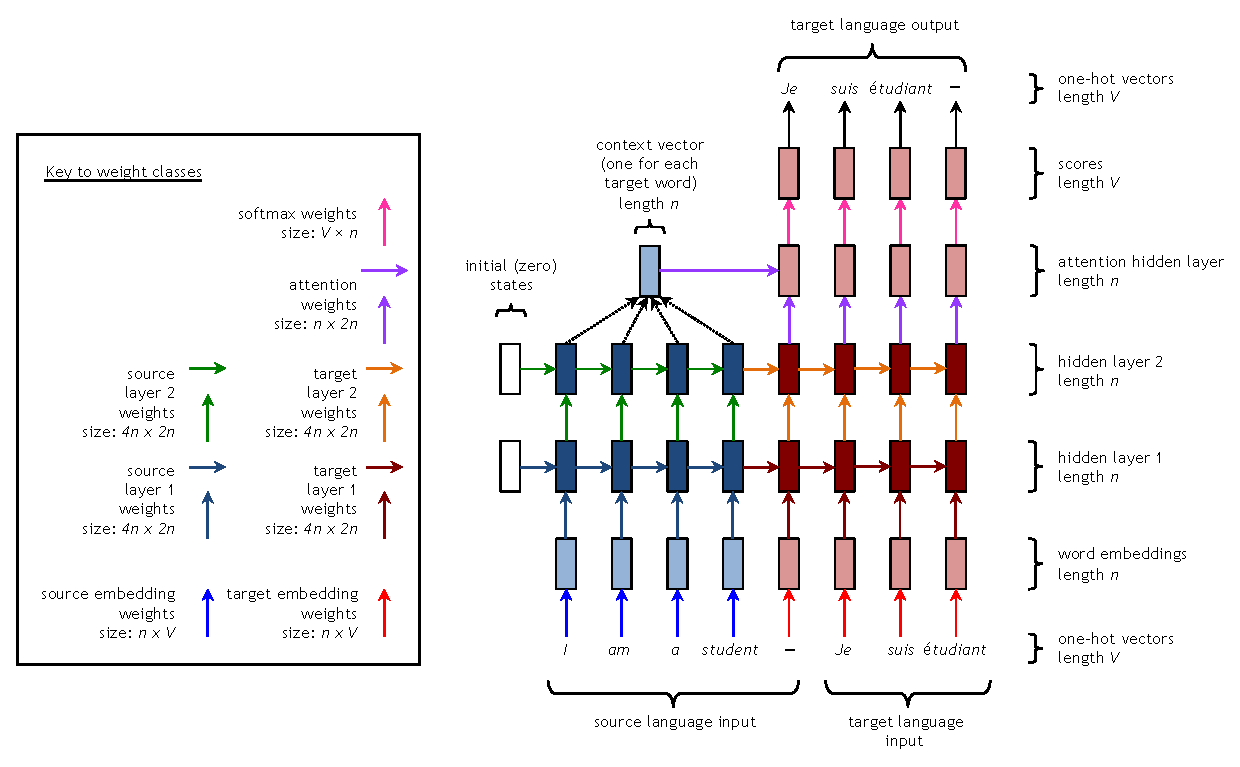
\includegraphics[width=\textwidth]{img/6-2_nmt_complex} %trim = 27mm 60mm 45mm 35mm, clip, 
\caption{NMT architecture. This example has two layers, but our system has four. The different weight classes are indicated by arrows of different color (the black arrows in the top right represent simply choosing the highest-scoring word, and thus require no parameters).
Best viewed in color.
}
\label{fig:nmt_complex}
\end{figure*}


Most of the above work has focused on compressing CNNs for vision tasks. 
We extend the magnitude-based pruning approach of \cite{han2015learning} to recurrent neural networks (RNN), in particular LSTM architectures for NMT, and to our knowledge we are the first to do so.
There has been some recent work on compression for RNNs \cite{lu2016learning,prabhavalkar2016compression}, but it focuses on other, non-pruning compression techniques. 
Nonetheless, our general observations on the distribution of redundancy in a
LSTM, detailed in Section \ref{subsubsec:redundancy}, are corroborated by \cite{lu2016learning}.




\subsection{Our Approach}
\label{subsec:approach}
\subsubsection{Understanding NMT Weights}
\label{subsubsec:lstm}
\begin{figure*}[t]
\centering
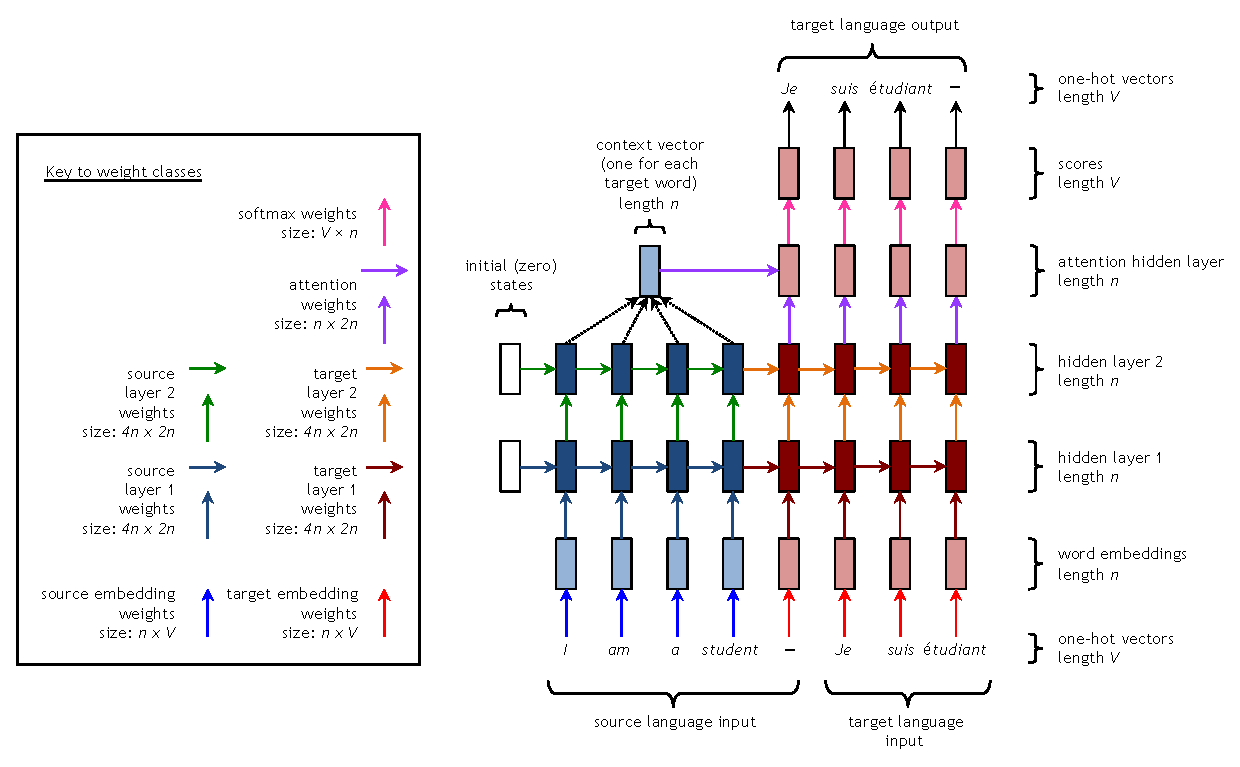
\includegraphics[width=\textwidth]{img/6-2_nmt_complex} %trim = 27mm 60mm 45mm 35mm, clip, 
\caption[Weights of NMT architecture]{NMT architecture. This example has two layers, but my system has four. The different weight classes are indicated by arrows of different color (the black arrows in the top right represent simply choosing the highest-scoring word, and thus require no parameters).
Best viewed in color.
}
\label{fig:nmt_complex}
\end{figure*}

In this work, I am focusing on the {\it deep multi-layer recurrent} architecture with {\it
LSTM} as the hidden unit type.
Figure~\ref{fig:nmt_complex} shows the system in detail,
highlighting the different types of parameters, or weights, in the model.
I will go through the architecture from bottom to top.
First, a vocabulary is chosen for each language, assuming that the top $V$ frequent
words are selected.
Thus, every word in the source or target vocabulary can be represented by a one-hot vector of length $V$.
The source input sentence and target input sentence, represented as a sequence
of one-hot vectors, are transformed into a sequence of word embeddings by the
\emph{embedding} weights. 
These embedding weights, which are learned during training, are different for the source words and the target words.
The word embeddings and all hidden layers are vectors of length $n$ (a chosen hyperparameter).

The word embeddings are then fed as input into the main network, which consists
of two multi-layer RNNs `stuck together' --- an encoder for the source
language and a decoder for the target language, each with their own
weights. 
The \emph{feed-forward} (vertical) weights connect
the hidden unit from the layer below to the upper RNN block, and the
\emph{recurrent} (horizontal) weights connect the hidden unit from the previous
time-step RNN block to the current time-step RNN block.
The hidden state at the top layer of the decoder is fed through an
\textit{attention} layer, which guides the translation by `paying attention'
to relevant parts of the source sentence.
Finally, for each target word, the top layer hidden unit is transformed by the
\emph{softmax} weights into a score vector of length $V$. The target word with the highest score is selected as the output translation.

{\it Weight Subgroups in LSTM} -- For the aforementioned RNN block, I choose to
use LSTM as the hidden unit type. To facilitate my later discussion 
on the different subgroups of weights
within LSTM, recall the details of the LSTM presented in Chapter 2 (2.35-2.37):
\begin{align}
\begin{pmatrix}
i\\
f\\
o\\
\hat{h}
\end{pmatrix}
&=
\begin{pmatrix}
\text{sigm}\\
\text{sigm}\\
\text{sigm}\\
\text{tanh}
\end{pmatrix}
T_{4n,2n}
\begin{pmatrix}
h_t^{l-1}\\
h_{t-1}^l
\end{pmatrix} \label{eqn:lstm_1} \\
c_t^l&=f \circ c_{t-1}^l + i \circ \hat{h} \label{eqn:lstm_2} \\
h_t^l &= o \circ \text{tanh}(c_t^l) \label{eqn:lstm_3}
\end{align}
Each LSTM block at time $t$ and layer $l$ computes as output a pair of
hidden and memory vectors ($h_t^l$, $c_t^l$) given the previous pair
($h_{t-1}^l$, $c_{t-1}^l$) and an input vector $h_t^{l-1}$ (either from the LSTM block below or
the embedding weights if $l\!=\!1$). All of these vectors
have length $n$.
The core of a LSTM block is the weight matrix $T_{4n,2n}$ of size $4n \times
2n$. This matrix can be decomposed into 8 subgroups that are responsible for the
interactions between $\{$input gate $i$, forget gate $f$, output gate $o$,
input signal $\hat{h}\} \times \{$feed-forward input $h_t^{l-1}$, recurrent
input $h_{t-1}^l\}$.

%\subsection{Evaluation metrics}
%I evaluate my models by two measures: BLEU score and perplexity. 
%BLEU compares the output target sentence with the human-translated target sentence, and is measured on a scale from 0 (worst) to 100 (best).
%Perplexity is the exponential of the average loss per word, measured on a scale from 1 (best) to infinity (worst). 
%%For each output target word, the model produces scores for each word in the vocabulary, which are converted to a probability distribution over the vocabulary. 
%The \emph{loss} is the negative log probability of the correct word --- that is, the lower the system's certainty in choosing the correct word, the higher the loss.
%
%Both evaluation metrics are valuable. 
%BLEU measures a system's performance on the end-goal of machine translation, translation quality, whereas perplexity is the quantity minimized during training.
%BLEU is a `hard' measure of performance, as it is calculated based on the sentences produced by the network, whereas perplexity is a `softer', more fine-grained measure that takes into account not just whether the correct target word was produced, but the probability of producing the correct target word.
%I use both BLEU and perplexity in this paper, as appropriate.

\subsubsection{Pruning Schemes}
\label{subsubsec:approach_schemes}
I follow the general magnitude-based approach of \cite{han2015learning}, which consists of pruning weights with smallest absolute value. However, I question the authors' pruning scheme with respect to the different weight classes, and experiment with three pruning schemes.
Suppose I wish to prune $x$\% of the total parameters in the model. 
How do I distribute the pruning over the different weight classes (illustrated in Figure~\ref{fig:nmt_complex}) of my model? 
I propose to examine three different pruning schemes:
\begin{enumerate}
\item \textit{Class-blind}: 
Take all parameters, sort them by magnitude and prune the $x$\% with smallest magnitude, regardless of weight class.
(So some classes are pruned proportionally more than others).
\item \textit{Class-uniform}: 
Within each class, sort the weights by magnitude and prune the $x$\% with smallest magnitude.
(So all classes have exactly $x$\% of their parameters pruned).
\item \textit{Class-distribution}: 
 For each class $c$, weights with magnitude less than $\lambda \sigma_c$ are
 pruned. Here, $\sigma_c$ is the standard deviation of that class and $\lambda$ is a universal parameter chosen such that in total, $x\%$ of all parameters are pruned.
This is used by \cite{han2015learning}.
\end{enumerate}
All these schemes have their seeming advantages.
Class-blind pruning is the simplest and adheres to the principle that pruning
weights (or equivalently, setting them to zero) is least damaging when
those weights are small, regardless of their locations in the architecture.
Class-uniform pruning and class-distribution pruning both seek to prune
proportionally within each weight class, either absolutely, or relative to the
standard deviation of that class.
I find that class-blind pruning outperforms both other schemes (see
Section~\ref{subsubsec:exp_schemes}).

\subsubsection{Retraining}
\label{subsubsec:approach_retraining}
In order to prune NMT models aggressively without performance loss, I retrain my pruned networks. 
That is, I continue to train the remaining weights, but maintain the sparse structure introduced by pruning.
In my implementation, pruned weights are represented by zeros in the weight matrices, 
and I use binary `mask' matrices, which represent the sparse structure of a network, 
to ignore updates to weights at pruned locations.
This implementation has the advantage of simplicity as it requires minimal changes to the training and deployment code, 
but I note that a more complex implementation utilizing sparse matrices and sparse matrix multiplication could potentially yield speed improvements.
However, such an implementation is beyond the scope of this work.

\begin{figure}
\centering
% !TEX root = acl2016.tex

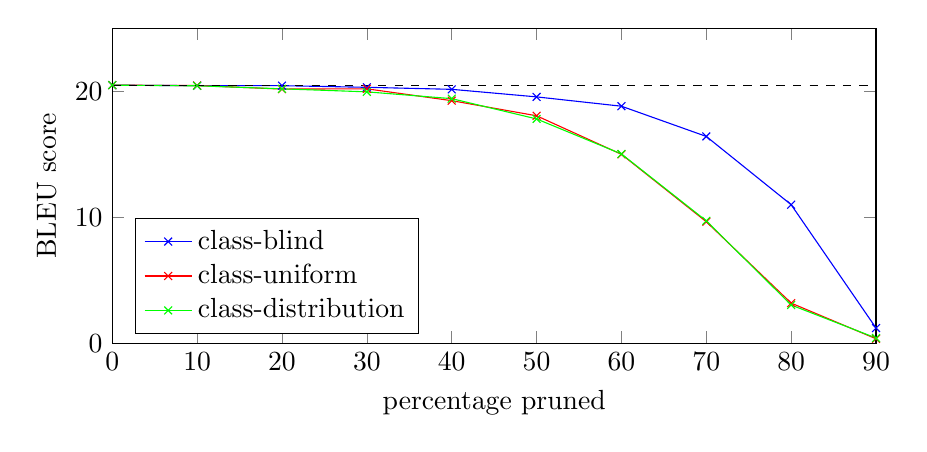
\begin{tikzpicture}

\begin{axis}[%
width=0.8\columnwidth,
height=4cm,
%at={(0\figurewidth,0\figureheight)},
scale only axis,
xmin=0,
xmax=90,
xtick={0, 10, 20, 30, 40, 50, 60, 70, 80, 90},
xlabel={percentage pruned},
%ymode=log,
ymin=0,
ymax=25,
yminorticks=true,
ylabel={BLEU score},
axis background/.style={fill=white},
legend pos = south west,
legend cell align=left
]
\addplot [color=blue,solid,mark=x,mark options={solid}]
  table[row sep=crcr]{%
  0	20.48\\
10	20.44\\
20	20.44\\
30	20.31\\
40	20.15\\
50	19.55\\
60	18.81\\
70	16.41\\
80	10.99\\
90	1.2\\
};
\addlegendentry{class-blind}

\addplot [color=red,solid,mark=x,mark options={solid}]
  table[row sep=crcr]{%
    0	20.48\\
10	20.45\\
20	20.17\\
30	20.19\\
40	19.25\\
50	18.05\\
60	14.99\\
70	9.64\\
80	3.18\\
90	0.35\\
};
\addlegendentry{class-uniform}

\addplot [color=green,solid,mark=x,mark options={solid}]
  table[row sep=crcr]{%
    0	20.48\\
10	20.43\\
20	20.19\\
30	19.95\\
40	19.41\\
50	17.8\\
60	15.02\\
70	9.71\\
80	3.03\\
90	0.41\\
};
\addlegendentry{class-distribution}

\addplot [color=black,dashed]
  table[row sep=crcr]{%
0	20.48\\
90	20.48\\
};
\end{axis}
\end{tikzpicture}%
\caption{Effects of different pruning schemes.}
\label{fig:pruning_methods}
\end{figure}

\begin{figure*}
\centering
% !TEX root = acl2016.tex


%\begin{tikzpicture}
%    \begin{axis}[
%width=0.8\textwidth,
%height=8cm,
%%at={(0\figurewidth,0\figureheight)},
%%scale only axis,
%        major y tick style = transparent,
%        xbar,
%        bar width=4pt,
%        xmajorgrids = true,
%        xlabel = {perplexity change},
%        symbolic y coords={source layer 1, source layer 2, source layer 3, source layer 4, target layer 1, target layer 2, target layer 3, target layer 4, attention, top layer, source embedding, target embedding},
%        ytick = data,
%        y=20pt,
%        scaled x ticks = false,
%     legend pos = south east,   
%    ]
%        \addplot[style={blue,fill=blue!50,mark=none}]
%            coordinates {(0.46659,source layer 1)  (0.362434,source layer 2)  (0.796254,source layer 3)  (0.794582,source layer 4)  (0.201001,target layer 1)  (0.222658,target layer 2)  (-0.291916,target layer 3)  (1.108432,target layer 4)  (0.4164,attention)  (7.803921,top layer)  (2.962925,source embedding)  (2.351362,target embedding)  };
%            
%        \addplot[style={red,fill=red!50,mark=none}]
%            coordinates {(0.471137,source layer 1)  (0.561763,source layer 2)  (1.829927,source layer 3)  (3.628541,source layer 4)  (0.422055,target layer 1)  (0.457759,target layer 2)  (0.473893,target layer 3)  (7.545939,target layer 4)  (6.362093,attention)  (16.277336,top layer)  (0.335614,source embedding)  (0.226382,target embedding)  };
%
%        \addplot[style={green,fill=green!50,mark=none}]
%            coordinates {(0.458798,source layer 1)  (0.543843,source layer 2)  (1.818222,source layer 3)  (3.93477,source layer 4)  (0.428267,target layer 1)  (0.46657,target layer 2)  (0.494273,target layer 3)  (8.308794,target layer 4)  (6.34294,attention)  (15.723167,top layer)  (0.311599,source embedding)  (0.253745,target embedding) };
%
%
%        \legend{delete smallest, uniform, standard deviation}
%    \end{axis}
%\end{tikzpicture}




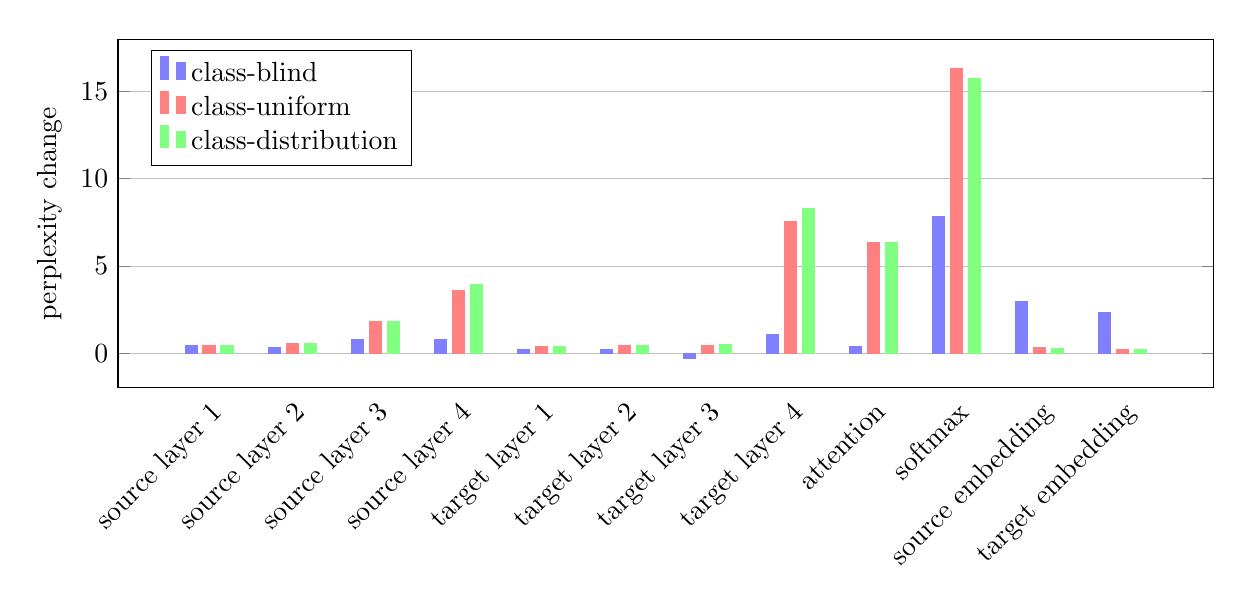
\begin{tikzpicture}
    \begin{axis}[
width=\textwidth,
height=6cm,
%at={(0\figurewidth,0\figureheight)},
%scale only axis,
        major x tick style = transparent,
        ybar,
        bar width=4.5pt,
        ymajorgrids = true,
        ylabel = {perplexity change},
        symbolic x coords={source layer 1, source layer 2, source layer 3, source layer 4, target layer 1, target layer 2, target layer 3, target layer 4, attention, softmax, source embedding, target embedding},
        x tick label style={rotate=45, anchor=north east, inner sep=0mm}, % inner sep controls how close the labels are to the plot
        xtick = data,
        x=30pt, % gap between groups of bars
        scaled y ticks = false,
     legend pos = north west,   
     legend cell align = left,
    ]
        \addplot[style={blue!50,fill=blue!50,mark=none}]
            coordinates {(source layer 1,0.46659)  (source layer 2,0.362434)  (source layer 3,0.796254)  (source layer 4,0.794582)  (target layer 1,0.201001)  (target layer 2,0.222658)  (target layer 3,-0.291916)  (target layer 4,1.108432)  (attention,0.4164)  (softmax,7.803921)  (source embedding,2.962925)  (target embedding,2.351362)};
            
        \addplot[style={red!50,fill=red!50,mark=none}]
            coordinates {(source layer 1,0.471137)  (source layer 2,0.561763)  (source layer 3,1.829927)  (source layer 4,3.628541)  (target layer 1,0.422055)  (target layer 2,0.457759)  (target layer 3,0.473893)  (target layer 4,7.545939)  (attention,6.362093)  (softmax,16.277336)  (source embedding,0.335614)  (target embedding,0.226382) };

        \addplot[style={green!50,fill=green!50,mark=none}]
            coordinates {(source layer 1,0.458798)  (source layer 2,0.543843)  (source layer 3,1.818222)  (source layer 4,3.93477)  (target layer 1,0.428267)  (target layer 2,0.46657)  (target layer 3,0.494273)  (target layer 4,8.308794)  (attention,6.34294)  (softmax,15.723167)  (source embedding,0.311599)  (target embedding,0.253745) 
 };
        \legend{class-blind, class-uniform, class-distribution}
    \end{axis}
\end{tikzpicture}
\caption[`Breakdown' of performance loss]{`Breakdown' of performance loss (i.e., perplexity increase) by weight class, when pruning 90\% of weights using each of the three pruning schemes. Each of the first eight classes have 8 million weights, attention has 2 million, and the last three have 50 million weights each.}
\label{fig:breakdown}
\end{figure*}




\begin{figure}
\centering
% !TEX root = acl2016.tex

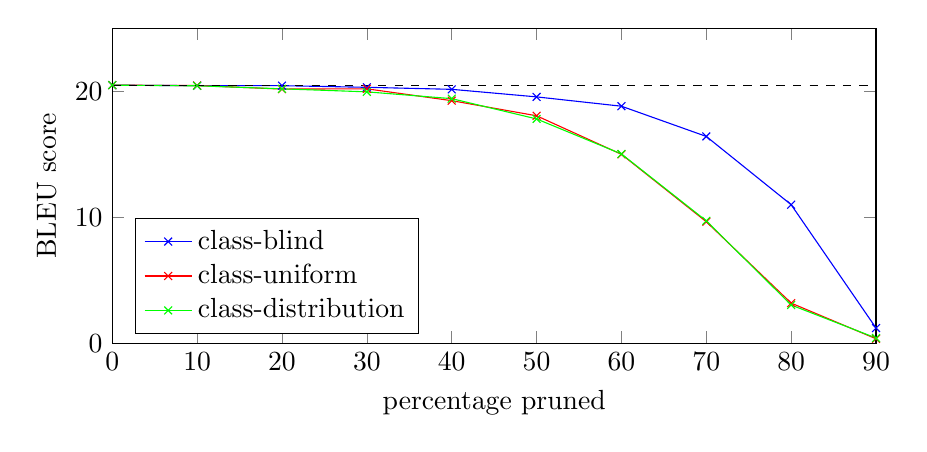
\begin{tikzpicture}

\begin{axis}[%
width=0.8\columnwidth,
height=4cm,
%at={(0\figurewidth,0\figureheight)},
scale only axis,
xmin=0,
xmax=90,
xtick={0, 10, 20, 30, 40, 50, 60, 70, 80, 90},
xlabel={percentage pruned},
%ymode=log,
ymin=0,
ymax=25,
yminorticks=true,
ylabel={BLEU score},
axis background/.style={fill=white},
legend pos = south west,
legend cell align=left
]
\addplot [color=blue,solid,mark=x,mark options={solid}]
  table[row sep=crcr]{%
  0	20.48\\
10	20.44\\
20	20.44\\
30	20.31\\
40	20.15\\
50	19.55\\
60	18.81\\
70	16.41\\
80	10.99\\
90	1.2\\
};
\addlegendentry{class-blind}

\addplot [color=red,solid,mark=x,mark options={solid}]
  table[row sep=crcr]{%
    0	20.48\\
10	20.45\\
20	20.17\\
30	20.19\\
40	19.25\\
50	18.05\\
60	14.99\\
70	9.64\\
80	3.18\\
90	0.35\\
};
\addlegendentry{class-uniform}

\addplot [color=green,solid,mark=x,mark options={solid}]
  table[row sep=crcr]{%
    0	20.48\\
10	20.43\\
20	20.19\\
30	19.95\\
40	19.41\\
50	17.8\\
60	15.02\\
70	9.71\\
80	3.03\\
90	0.41\\
};
\addlegendentry{class-distribution}

\addplot [color=black,dashed]
  table[row sep=crcr]{%
0	20.48\\
90	20.48\\
};
\end{axis}
\end{tikzpicture}%
\caption{Effects of different pruning schemes.}
\label{fig:pruning_methods}
\end{figure}

\begin{figure*}
\centering
% !TEX root = acl2016.tex


%\begin{tikzpicture}
%    \begin{axis}[
%width=0.8\textwidth,
%height=8cm,
%%at={(0\figurewidth,0\figureheight)},
%%scale only axis,
%        major y tick style = transparent,
%        xbar,
%        bar width=4pt,
%        xmajorgrids = true,
%        xlabel = {perplexity change},
%        symbolic y coords={source layer 1, source layer 2, source layer 3, source layer 4, target layer 1, target layer 2, target layer 3, target layer 4, attention, top layer, source embedding, target embedding},
%        ytick = data,
%        y=20pt,
%        scaled x ticks = false,
%     legend pos = south east,   
%    ]
%        \addplot[style={blue,fill=blue!50,mark=none}]
%            coordinates {(0.46659,source layer 1)  (0.362434,source layer 2)  (0.796254,source layer 3)  (0.794582,source layer 4)  (0.201001,target layer 1)  (0.222658,target layer 2)  (-0.291916,target layer 3)  (1.108432,target layer 4)  (0.4164,attention)  (7.803921,top layer)  (2.962925,source embedding)  (2.351362,target embedding)  };
%            
%        \addplot[style={red,fill=red!50,mark=none}]
%            coordinates {(0.471137,source layer 1)  (0.561763,source layer 2)  (1.829927,source layer 3)  (3.628541,source layer 4)  (0.422055,target layer 1)  (0.457759,target layer 2)  (0.473893,target layer 3)  (7.545939,target layer 4)  (6.362093,attention)  (16.277336,top layer)  (0.335614,source embedding)  (0.226382,target embedding)  };
%
%        \addplot[style={green,fill=green!50,mark=none}]
%            coordinates {(0.458798,source layer 1)  (0.543843,source layer 2)  (1.818222,source layer 3)  (3.93477,source layer 4)  (0.428267,target layer 1)  (0.46657,target layer 2)  (0.494273,target layer 3)  (8.308794,target layer 4)  (6.34294,attention)  (15.723167,top layer)  (0.311599,source embedding)  (0.253745,target embedding) };
%
%
%        \legend{delete smallest, uniform, standard deviation}
%    \end{axis}
%\end{tikzpicture}




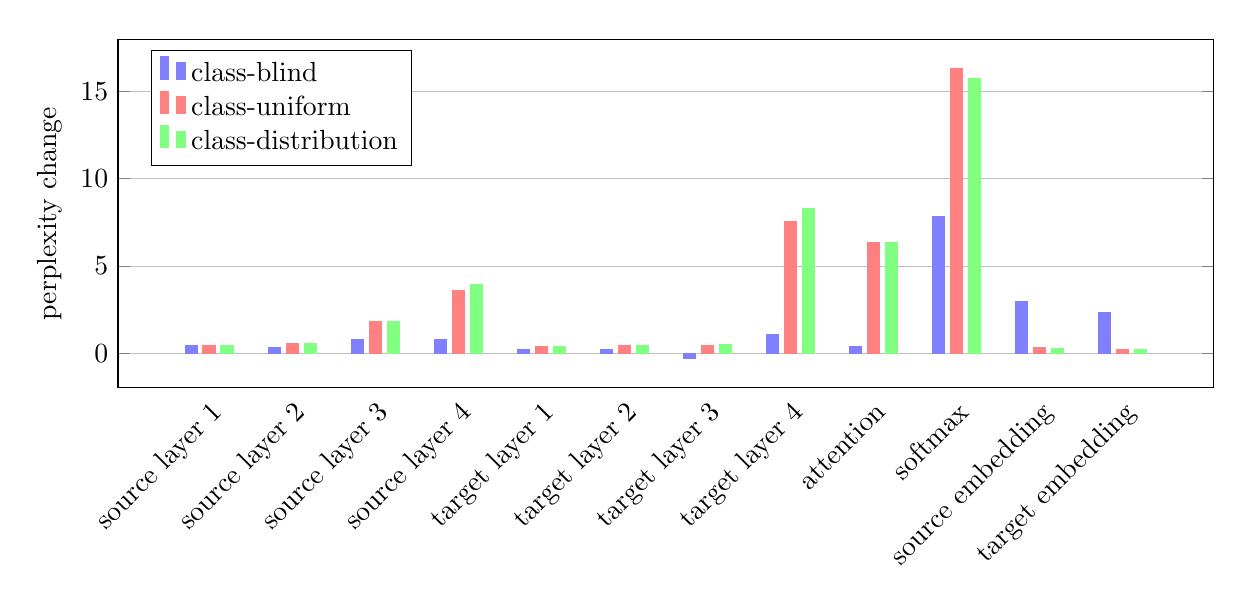
\begin{tikzpicture}
    \begin{axis}[
width=\textwidth,
height=6cm,
%at={(0\figurewidth,0\figureheight)},
%scale only axis,
        major x tick style = transparent,
        ybar,
        bar width=4.5pt,
        ymajorgrids = true,
        ylabel = {perplexity change},
        symbolic x coords={source layer 1, source layer 2, source layer 3, source layer 4, target layer 1, target layer 2, target layer 3, target layer 4, attention, softmax, source embedding, target embedding},
        x tick label style={rotate=45, anchor=north east, inner sep=0mm}, % inner sep controls how close the labels are to the plot
        xtick = data,
        x=30pt, % gap between groups of bars
        scaled y ticks = false,
     legend pos = north west,   
     legend cell align = left,
    ]
        \addplot[style={blue!50,fill=blue!50,mark=none}]
            coordinates {(source layer 1,0.46659)  (source layer 2,0.362434)  (source layer 3,0.796254)  (source layer 4,0.794582)  (target layer 1,0.201001)  (target layer 2,0.222658)  (target layer 3,-0.291916)  (target layer 4,1.108432)  (attention,0.4164)  (softmax,7.803921)  (source embedding,2.962925)  (target embedding,2.351362)};
            
        \addplot[style={red!50,fill=red!50,mark=none}]
            coordinates {(source layer 1,0.471137)  (source layer 2,0.561763)  (source layer 3,1.829927)  (source layer 4,3.628541)  (target layer 1,0.422055)  (target layer 2,0.457759)  (target layer 3,0.473893)  (target layer 4,7.545939)  (attention,6.362093)  (softmax,16.277336)  (source embedding,0.335614)  (target embedding,0.226382) };

        \addplot[style={green!50,fill=green!50,mark=none}]
            coordinates {(source layer 1,0.458798)  (source layer 2,0.543843)  (source layer 3,1.818222)  (source layer 4,3.93477)  (target layer 1,0.428267)  (target layer 2,0.46657)  (target layer 3,0.494273)  (target layer 4,8.308794)  (attention,6.34294)  (softmax,15.723167)  (source embedding,0.311599)  (target embedding,0.253745) 
 };
        \legend{class-blind, class-uniform, class-distribution}
    \end{axis}
\end{tikzpicture}
\caption{`Breakdown' of performance loss (i.e., perplexity increase) by weight class, when pruning 90\% of weights using each of the three pruning schemes. Each of the first eight classes have 8 million weights, attention has 2 million, and the last three have 50 million weights each.}
\label{fig:breakdown}
\end{figure*}

\subsection{Experiments}
\label{subsec:exp}
% !TEX root = acl2016.tex

We evaluate the effectiveness of our pruning approaches on a state-of-the-art
NMT model.\footnote{We thank the authors of \cite{luong2015effective}
for providing their trained models and assistance in using the codebase
at \url{https://github.com/lmthang/nmt.matlab}.} 
Specifically, an attention-based English-German NMT system from
\cite{luong2015effective} is considered. 
%This system uses the global attention mechanism with the dot-product function and the input-feeding approach. 
Training data was obtained from WMT'14 consisting
of 4.5M sentence pairs (116M English words, 110M German words). For
more details on training hyperparameters, we refer readers to Section 4.1 of
\cite{luong2015effective}.
All models are tested on newstest2014 (2737 sentences). 
The model achieves a
perplexity of 6.1 and a BLEU score of
20.5 (after unknown word replacement).\footnote{The performance of this model
is reported under row {\it global (dot)} in Table 4 of
\cite{luong2015effective}.}

When {\it retraining} pruned NMT systems, we use the following settings: (a) we start
with a smaller learning rate of 0.5 (the original model uses a learning rate of
1.0), (b) we train for fewer epochs, 4 instead of 12, using plain SGD, (c) a simple learning
rate schedule is employed; after 2 epochs, we begin to halve the learning rate
every half an epoch, and (d) all other hyperparameters are the same, such as
mini-batch size 128, maximum gradient norm 5, and dropout with probability 0.2.

\subsubsection{Comparing pruning schemes}
\label{subsubsec:exp_schemes}
Despite its simplicity, we observe in Figure~\ref{fig:pruning_methods} that {\it
class-blind} pruning outperforms both other schemes in terms of translation
quality at all pruning percentages.
In order to understand this result, for each of the three pruning schemes, we pruned each class separately and recorded the effect on performance (as measured by perplexity).
Figure \ref{fig:breakdown} shows that with class-uniform pruning, the overall performance loss is caused disproportionately by a few classes: target layer 4, attention and softmax weights. Looking at Figure \ref{fig:scatter}, we see that the most damaging classes to prune also tend to be those with weights of greater magnitude --- these classes have much larger weights than others at the same percentile, so pruning them under the class-uniform pruning scheme is more damaging. The situation is similar for class-distribution pruning.



By contrast, Figure \ref{fig:breakdown} shows that under class-blind pruning, the damage caused by pruning softmax, attention and target layer 4 weights is greatly decreased, and the contribution of each class towards the performance loss is overall more uniform.
In fact, the distribution begins to reflect the number of parameters in each class --- for example, the source and target embedding classes have larger contributions because they have more weights. 
We use only class-blind pruning for the rest of the experiments.

Figure \ref{fig:breakdown} also reveals some interesting information about the distribution of redundancy in NMT architectures --- namely it seems that higher layers are more important than lower layers, and that attention and softmax weights are crucial. We will explore the distribution of redundancy further in Section \ref{subsec:redundancy}.

\begin{figure}
\centering
% !TEX root = acl2016.tex

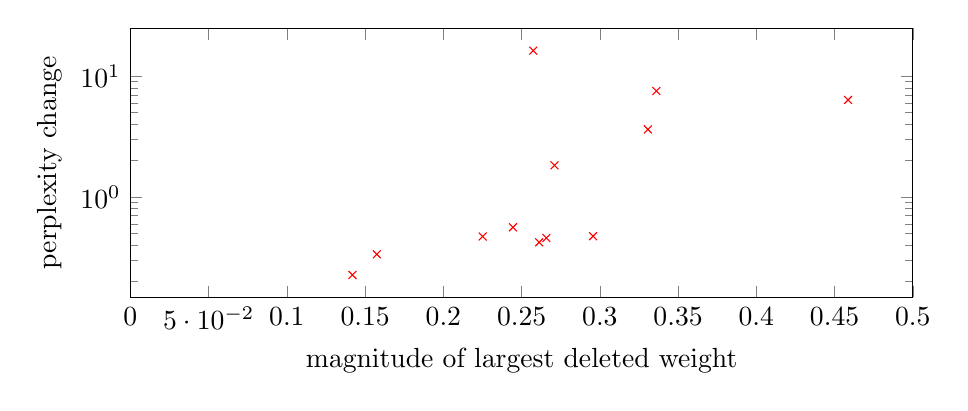
\begin{tikzpicture}
\begin{semilogyaxis}[
width=0.95\columnwidth,
height=5cm,
xlabel={magnitude of largest deleted weight}, 
ylabel={perplexity change},
xmin=0,
xmax=0.5,
]
\addplot[
only marks,
color=red,
mark=x,
]
table[row sep=crcr]
{
0.22513		0.471137\\
0.244492		0.561763\\
0.270999		1.829927\\
0.330704		3.628541\\
0.261247		0.422055\\
0.265832		0.457759\\
0.295644		0.473893\\
0.336088		7.545939\\
0.458583		6.362093\\
0.257479		16.277336\\
0.157486		0.335614\\
0.14194		0.226382\\
};
\end{semilogyaxis}
\end{tikzpicture}
\caption{Magnitude of largest deleted weight vs. perplexity change, for the 12 different weight classes when pruning 90\% of parameters by class-uniform pruning.}
\label{fig:scatter}
\end{figure}

\subsubsection{Pruning and retraining}
\label{subsec:effect}


Pruning has an immediate negative impact on performance (as measured by BLEU) that is exponential in pruning percentage; this is demonstrated by the blue line in Figure \ref{fig:main_results}.
However we find that up to about 40\% pruning, performance is mostly unaffected, indicating a large amount of redundancy and over-parameterization in NMT.

We now consider the effect of retraining pruned models.
The orange line in Figure \ref{fig:main_results} shows that after retraining the pruned models, baseline performance (20.48 BLEU) is both recovered and improved upon, up to 80\% pruning (20.91 BLEU), with only a small performance loss at 90\% pruning (20.13 BLEU).
This may seem surprising, as we might not expect a sparse model to significantly out-perform a model with five times as many parameters.
There are several possible explanations, two of which are given below.
\begin{figure}
\centering
% !TEX root = acl2016.tex

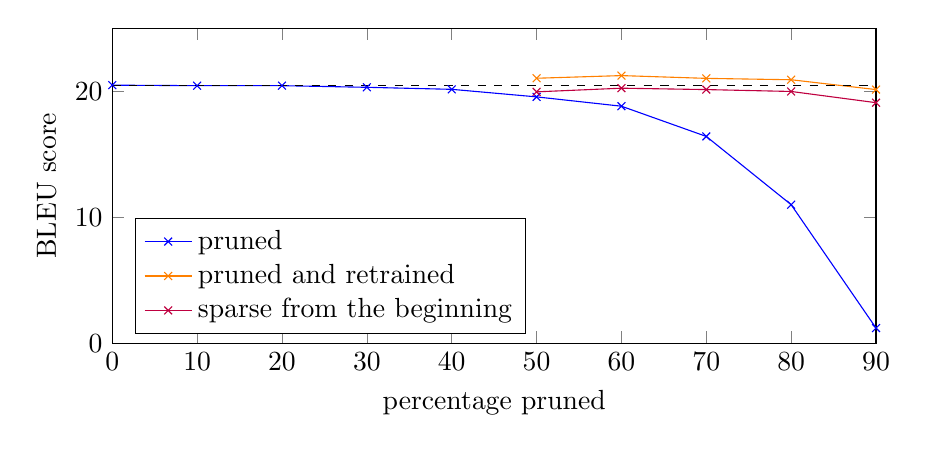
\begin{tikzpicture}

\begin{axis}[%
width=0.8\columnwidth,
height=4cm,
scale only axis,
xmin=0,
xmax=90,
xtick={0,10, 20, 30, 40, 50, 60, 70, 80, 90},
xlabel={percentage pruned},
ymin=0,
ymax=25,
yminorticks=true,
ylabel={BLEU score},
axis background/.style={fill=white},
legend pos = south west,
legend cell align=left,
]
\addplot [color=blue,solid,mark=x,mark options={solid}]
  table[row sep=crcr]{%
  0	20.48\\
10	20.44\\
20	20.44\\
30	20.31\\
40	20.15\\
50	19.55\\
60	18.81\\
70	16.41\\
80	10.99\\
90	1.2\\
};
\addlegendentry{pruned}

\addplot [color=orange,solid,mark=x,mark options={solid}]
  table[row sep=crcr]{%
50	21.03\\
60	21.24\\
70	21.02\\
80	20.91\\
90	20.13\\
};
\addlegendentry{pruned and retrained}

\addplot [color=purple,solid,mark=x,mark options={solid}]
  table[row sep=crcr]{%
50	19.95\\
60	20.24\\
70	20.13\\
80	19.98\\
90	19.09\\
};
\addlegendentry{sparse from the beginning}

\addplot [color=black,dashed]
  table[row sep=crcr]{%
0	20.48\\
90	20.48\\
};
\end{axis}
\end{tikzpicture}%
\caption{Performance of pruned models (a) after pruning, (b) after pruning and retraining, and (c) when trained with sparsity structure from the outset (see Section \ref{sec:sparse}).}
\label{fig:main_results}
\end{figure}

Firstly, we found that the less-pruned models perform better on the training set than the validation set, whereas the more-pruned models have closer performance on the two sets. 
This indicates that pruning has a regularizing effect on the retraining phase, though clearly more is not always better, as the 50\% pruned and retrained model has better validation set performance than the 90\% pruned and retrained model.
Nonetheless, this regularization effect may explain why the pruned and retrained models outperform the baseline.
\begin{figure}[tbh]
\centering
% !TEX root = acl2016.tex

\begin{tikzpicture}

\begin{axis}[%
width=0.8\columnwidth,
height=4cm,
scale only axis,
xmin=0,
xmax=540000,
%xtick={},
xlabel={training iterations},
ymin=1,
ymax=8,
yminorticks=true,
ylabel={loss},
axis background/.style={fill=white},
%legend pos = south west,
%legend cell align=left
]

\addplot [color=black,dotted]
  table[row sep=crcr]{%
0	2.27\\
540000	2.27\\
};

\addplot [color=black,dotted]
  table[row sep=crcr]{%
405000	0\\
405000	8\\
};

\addplot [color=blue,solid,mark options={solid}]
  table[row sep=crcr]{%
5000	6.89\\
10000	5.91\\
15000	5.34\\
20000	4.88\\
25000	4.35\\
30000	3.9\\
35000	3.66\\
40000	3.61\\
45000	3.55\\
50000	3.5\\
55000	3.43\\
60000	3.3\\
65000	3.16\\
70000	3.07\\
75000	3.06\\
80000	3.05\\
85000	3.04\\
90000	3.01\\
95000	2.94\\
100000	2.86\\
105000	2.82\\
110000	2.82\\
115000	2.82\\
120000	2.81\\
125000	2.8\\
130000	2.75\\
135000	2.7\\
140000	2.67\\
145000	2.67\\
150000	2.67\\
155000	2.67\\
160000	2.66\\
165000	2.63\\
170000	2.59\\
175000	2.57\\
180000	2.57\\
185000	2.57\\
190000	2.57\\
195000	2.57\\
200000	2.54\\
205000	2.51\\
210000	2.5\\
215000	2.5\\
220000	2.5\\
225000	2.5\\
230000	2.5\\
235000	2.48\\
240000	2.45\\
245000	2.44\\
250000	2.44\\
255000	2.44\\
260000	2.44\\
265000	2.44\\
270000	2.42\\
275000	2.4\\
280000	2.39\\
285000	2.39\\
290000	2.4\\
295000	2.4\\
300000	2.4\\
305000	2.38\\
310000	2.36\\
315000	2.35\\
320000	2.35\\
325000	2.36\\
330000	2.36\\
335000	2.35\\
340000	2.34\\
345000	2.32\\
350000	2.31\\
355000	2.31\\
360000	2.31\\
365000	2.31\\
370000	2.31\\
375000	2.29\\
380000	2.28\\
385000	2.27\\
390000	2.27\\
395000	2.27\\
400000	2.27\\
405000	2.27\\
410000	2.53\\
415000	2.52\\
420000	2.48\\
425000	2.42\\
430000	2.22\\
435000	2.05\\
440000	1.99\\
445000	2.04\\
450000	2.08\\
455000	2.11\\
460000	2.12\\
465000	2.06\\
470000	1.99\\
475000	1.96\\
480000	1.99\\
485000	2.02\\
490000	2.03\\
495000	2.04\\
500000	2.01\\
505000	1.96\\
510000	1.95\\
515000	1.97\\
520000	1.98\\
525000	2\\
530000	2\\
535000	1.98\\
540000	1.95\\
};

\end{axis}
\end{tikzpicture}%
\caption{The validation set loss during training, pruning and retraining. The vertical dotted line marks the point when 80\% of the parameters are pruned. The horizontal dotted line marks the best performance of the unpruned baseline.}
\label{fig:loss_curve}
\end{figure}

\begin{figure*}
\centering
\includegraphics[trim = 0mm 130mm 300mm 0mm, clip, width=\textwidth]{img/6-2_redundancy_good}
\caption{Graphical representation of the location of small weights in various parts of the model. 
Black pixels represent weights with absolute size in the bottom 80\%; white pixels represent those with absolute size in the top 20\%.
Equivalently, these pictures illustrate which parameters remain after pruning 80\% using our class-blind pruning scheme.
}
\label{fig:redundancy_location}
\end{figure*}



Alternatively, pruning may serve as a means to escape a local optimum. 
Figure \ref{fig:loss_curve} shows the loss function over time during the training, pruning and retraining process.
During the original training process, the loss curve flattens out and seems to converge (note that we use early stopping to obtain our baseline model, so the original model was trained for longer than shown in Figure \ref{fig:loss_curve}).
Pruning causes an immediate increase in the loss function, but enables further gradient descent, allowing the retraining process to find a new, better local optimum.
It seems that the disruption caused by pruning is beneficial in the long-run.

\subsubsection{Starting with sparse models}
\label{subsec:sparse}
The favorable performance of the pruned and retrained models raises the question: can we get a shortcut to this performance by \emph{starting} with sparse models?
That is, rather than train, prune, and retrain, what if we simply prune then train?
To test this, we took the sparsity structure of our 50\%--90\% pruned models, and trained completely new models with the same sparsity structure.
The purple line in Figure \ref{fig:main_results} shows that the `sparse from the beginning' models do not perform as well as the pruned and retrained models, but they do come close to the baseline performance.
This shows that while the sparsity structure alone contains useful information about redundancy and can therefore produce a competitive compressed model, it is important to interleave pruning with training.

Though our method involves just one pruning stage, other pruning methods interleave pruning with training more closely by including several iterations \cite{collins2014memory,han2015learning}.
We expect that implementing this for NMT would likely result in further compression and performance improvements.



\subsubsection{Storage size}
The original unpruned model (a MATLAB file) has size 782MB.
The 80\% pruned and retrained model is 272MB, which is a 65.2\% reduction.
In this work we focus on compression in terms of number of parameters rather than storage size, because it is invariant across implementations.

\subsubsection{Distribution of redundancy in NMT}
\label{subsubsec:redundancy}

We visualize in Figure~\ref{fig:redundancy_location} the redundancy structore of
our NMT baseline model.
{\it Black} pixels represent weights near to zero (those that can be pruned); {\it white} pixels represent larger ones.
First we consider the embedding weight matrices, whose columns correspond to words in the vocabulary.
Unsurprisingly, in Figure \ref{fig:redundancy_location}, we see that the parameters corresponding to the less common words are more dispensable.
In fact, at the 80\% pruning rate, for 100 uncommon source words and 1194
uncommon target words, we delete \emph{all} parameters corresponding to that word.
This is not quite the same as removing the word from the vocabulary --- true out-of-vocabulary words are mapped to the embedding for the `unknown word' symbol, whereas these `pruned-out' words are mapped to a zero embedding.
However in the original unpruned model these uncommon words already had near-zero embeddings, indicating that the model was unable to learn sufficiently distinctive representations.

Returning to Figure \ref{fig:redundancy_location}, now look at the eight weight matrices for the source and target connections at each of the four layers.
Each matrix corresponds to the $4n \times 2n$ matrix $T_{4n,2n}$ in Equation (\ref{eqn:lstm_1}).
In all eight matrices, we observe --- as does \cite{lu2016learning} --- that the weights connecting to the input $\hat{h}$ are most crucial, followed by the input gate $i$, then the output gate $o$, then the forget gate $f$. 
This is particularly true of the lower layers, which focus primarily on the input $\hat{h}$. 
However for higher layers, especially on the target side, weights connecting to the gates are as important as those connecting to the input $\hat{h}$.
The gates represent the LSTM's ability to add to, delete from or retrieve information from the memory cell.
Figure \ref{fig:redundancy_location} therefore shows that these sophisticated memory cell abilities are most important at the \emph{end} of the NMT pipeline (the top layer of the decoder).
This is reasonable, as we expect higher-level features to be learned later in a deep learning pipeline.

We also observe that for lower layers, the feed-forward input is much more important than the recurrent input, whereas for higher layers the recurrent input becomes more important.
This makes sense: lower layers concentrate on the low-level information from the current word embedding (the feed-forward input), whereas higher layers make use of the higher-level representation of the sentence so far (the recurrent input).

Lastly, on close inspection, we notice several white diagonals emerging within
some subsquares of the matrices in Figure \ref{fig:redundancy_location},
indicating that even without initializing the weights to identity matrices
(as is sometimes done \cite{le2015simple}),
an identity-like weight matrix is learned. At higher pruning percentages, these diagonals become more pronounced.

\subsection{Generalizability of our results}
To test the generalizability of our results, we also test our pruning approach
on a smaller, non-state-of-the-art NMT model trained on the WIT3 Vietnamese-English 
dataset \cite{cettoloEtAl:EAMT2012}, which consists of 133,000 sentence pairs.
This model is effectively a scaled-down version of the state-of-the-art model in \cite{luong2015effective},
with fewer layers, smaller vocabulary size, smaller hidden layer size, no attention mechanism,
and about 11\% as many parameters in total.
It achieves a BLEU score of 9.61 on the validation set.

Although this model and its training set are on a different scale to our main model, 
and the language pair is different, 
we found very similar results. 
For this model, it is possible to prune 60\% of parameters with no immediate performance loss,
and with retraining it is possible to prune 90\%, and regain original performance.
Our main observations from Sections \ref{subsec:exp_schemes} to \ref{subsec:redundancy}
are also replicated; in particular, class-blind pruning is most successful,
`sparse from the beginning' models are less successful than pruned and retrained models,
and we observe the same patterns as seen in Figure \ref{fig:redundancy_location}.



\subsection{Future Work}
As noted in Section \ref{sec:sparse}, including \emph{several} iterations of pruning and retraining would likely improve the compression and performance of our pruning method.
If possible it would be highly valuable to exploit the sparsity of the pruned models to speed up training and runtime, perhaps through sparse matrix representations and multiplications (see Section \ref{subsec:approach_retraining}).
Though we have found magnitude-based pruning to perform very well, it would be instructive to revisit the original claim that other pruning methods (for example Optimal Brain Damage and Optimal Brain Surgery) are more principled, and perform a comparative study.

\subsection{Conclusion}
\label{subsec:conclusion}
We have shown that weight pruning with retraining is a highly effective method of compression and regularization on a state-of-the-art NMT system, compressing the model to 20\% of its size with no loss of performance. 
Though we are the first to apply compression techniques to NMT, we obtain a similar degree of compression to other current work on compressing state-of-the-art deep neural networks, with an approach that is simpler than most.
We have found that the absolute size of parameters is of primary importance when choosing which to prune, leading to an approach that is extremely simple to implement, and can be applied to any neural network.
Lastly, we have gained insight into the distribution of redundancy in the NMT architecture.


\section{Future Outlook}

